%%%%%%%%%%%%%%%%%%%%%%%%%%%%%%%%%%%%%%%%%%%%%%%%%%%%%%%%%%%%%%%%%%%%%%%%%%%%%%%%%%%%%%%%%%%%%%%%%%%%%%%%%%%%%%%%%%%%%%%%%%%%%%%%%%%%%%%%%%%%%%%%%%%%%%%%%%%
% This is just an example/guide for you to refer to when submitting manuscripts to Frontiers, it is not mandatory to use Frontiers .cls files nor frontiers.tex  %
% This will only generate the Manuscript, the final article will be typeset by Frontiers after acceptance.   
% When submitting your files, remember to upload this *tex file, the pdf generated with it, the *bib file (if bibliography is not within the *tex) and all the figures.
%%%%%%%%%%%%%%%%%%%%%%%%%%%%%%%%%%%%%%%%%%%%%%%%%%%%%%%%%%%%%%%%%%%%%%%%%%%%%%%%%%%%%%%%%%%%%%%%%%%%%%%%%%%%%%%%%%%%%%%%%%%%%%%%%%%%%%%%%%%%%%%%%%%%%%%%%%%

%%% Version 3.4 Generated 2018/06/15 %%%
%%% You will need to have the following packages installed: datetime, fmtcount, etoolbox, fcprefix, which are normally inlcuded in WinEdt. %%%
%%% In http://www.ctan.org/ you can find the packages and how to install them, if necessary.
%%%  NB logo1.jpg is required in the path in order to correctly compile front page header %%%

\documentclass[utf8]{frontiersSCNS} % for Science, Engineering and Humanities and Social Sciences articles
%\documentclass[utf8]{frontiersHLTH} % for Health articles
%\documentclass[utf8]{frontiersFPHY} % for Physics and Applied Mathematics and Statistics articles

%\setcitestyle{square} % for Physics and Applied Mathematics and Statistics articles
\usepackage{url,hyperref,lineno,microtype,subcaption}
\usepackage[onehalfspacing]{setspace}
\usepackage{adjustbox}
\usepackage{graphicx}

\linenumbers
\doublespacing

% Leave a blank line between paragraphs instead of using \\

\def\keyFont{\fontsize{8}{11}\helveticabold }
\def\firstAuthorLast{Hu {et~al.}} %use et al only if is more than 1 author
\def\Authors{Shihao Hu\,$^{1}$, Yuzhi Lu$^{1}$, Andrea Tura\,$^{2}$, Giovanni Pacini\,$^{2}$, David Z. D’Argenio$^{1,*}$}
% Affiliations should be keyed to the author's name with superscript numbers and be listed as follows: Laboratory, Institute, Department, Organization, City, State abbreviation (USA, Canada, Australia), and Country (without detailed address information such as city zip codes or street names).
% If one of the authors has a change of address, list the new address below the correspondence details using a superscript symbol and use the same symbol to indicate the author in the author list.
\def\Address{$^{1}$Department of Biomedical Engineering, University of Southern California, Los Angeles, CA, USA \\
$^{2}$Metabolic Unit, CNR Institute of Neuroscience, Corso Stati Uniti 4, 35127 Padova, Italy}
% The Corresponding Author should be marked with an asterisk
% Provide the exact contact address (this time including street name and city zip code) and email of the corresponding author
\def\corrAuthor{David Z. D’Argenio}

\def\corrEmail{dargenio@usc.edu}

\begin{document}
\onecolumn
\firstpage{1}

\title[Hierarchical Modeling  of Glucose Effectiveness]{An Analysis of Glucose Effectiveness in Subjects with Normal Glucose Tolerance and Type 2 Diabetes via Hierarchical Modeling} 

\author[\firstAuthorLast ]{\Authors} %This field will be automatically populated
\address{} %This field will be automatically populated
\correspondance{} %This field will be automatically populated

\extraAuth{}% If there are more than 1 corresponding author, comment this line and uncomment the next one.
%\extraAuth{corresponding Author2 \\ Laboratory X2, Institute X2, Department X2, Organization X2, Street X2, City X2 , State XX2 (only USA, Canada and Australia), Zip Code2, X2 Country X2, email2@uni2.edu}

\maketitle
Number of words:  \\
Number of figures and tables: 8

\begin{abstract}
\section{}
abstract contents
% All article types require a minimum of 5 and a maximum of 8 keywords.

% For full guidelines regarding your manuscript please refer to \href{http://www.frontiersin.org/about/AuthorGuidelines}{Author Guidelines}.
% As a primary goal, the abstract should render the general significance and conceptual advance of the work clearly accessible to a broad readership. References should not be cited in the abstract. Leave the Abstract empty if your article does not require one, please see \href{http://www.frontiersin.org/about/AuthorGuidelines#SummaryTable}{Summary Table} for details according to article type. 

\tiny
 \keyFont{ \section{Keywords:} intravenous glucose tolerance test, keyword, keyword, keyword, keyword, keyword, keyword, keyword} %All article types: you may provide up to 8 keywords; at least 5 are mandatory.
\end{abstract}

\section{INTRODUCTION} % Succinct, with no subheadings
% 1. glucose intolerance, SG importance, modulation of SG and its impact, physiologic of SG, therapy based on SG
%Glucose intolerance, as determined by a combined interaction of insulin secretion, insulin action and glucose effectiveness ($S_G$), is a universal characteristic of both type 1 diabetes and type 2 diabetes (T2D). Among the three components, glucose effectiveness is defined as the ability of glucose itself to increase glucose utilization and inhibit hepatic glucose production, via mass action effects and other mechanisms \citep{Dube2015}. Compared to insulin effects, glucose effectiveness exerts earlier influence to maintain normoglycemia. It was reported that, in normal subjects, glucose effectiveness independent of insulin accounts for 45\% to 65\% of the total glucose disposal after an intravenous glucose load \citep{Alford_2018}. In patients with defective insulin production and action (e.g., diabetes), the contribution of insulin is minimal and thus, $S_G$ mediated glucose disposition will dominate \citep{Dube2015}. The potential application of $S_G$ as the predictor and therapeutic target of glucose intolerance and T2D has been mentioned before (\citet{basu_2009}, \citet{pau_2014}, \citet{Alford_2018}). However, despite the equal or greater importance of glucose effectiveness, previous research has been mainly focused on impaired insulin secretion function and insulin resistance as important factors of glucose intolerance or diabetes, rather than glucose effectiveness \citep{Alford_2018}. Although limited investigations that quantify $S_G$ have reported decreased $S_G$ in T2D, there still exists some inconsistencies, probably due to the differences in experiments and limited subjects included in the analysis \citep{Dube2015}. 
Glucose intolerance is determined by a combined interaction of insulin secretion, insulin action and glucose effectiveness. Glucose effectiveness, defined as the ability of glucose itself to increase glucose utilization and inhibit hepatic glucose production via mass action effects and other mechanisms \citep{Dube2015}, exerts an earlier temporal influence relative to insulin effects in maintaining normoglycemia. In normal subjects, it has been reported that glucose effectiveness independent of insulin accounts for 45\% to 65\% of the total glucose disposal following an intravenous glucose load \citep{Alford_2018}. In patients with defective insulin production and action, the contribution of insulin to glucose disposition is limited, and thus glucose effectiveness will be a crucial component to maintain normal glucose tolerance \citep{Dube2015}. Given its central role in glucose homeostasis, glucose effectiveness has been proposed as an important indicator of glucose intolerance and as a therapeutic target for treating patients with impaired glucose regulation (\citet{basu_2009}, \citet{pau_2014}, \citet{Alford_2018}). However, there have been only limited studies aimed at quantifying glucose effectiveness in subjects with normal and impaired glucose tolerance, and there are inconsistencies in those studies that have been reported, in part due to  differences in experiments and limited subjects included in the analysis \citep{Dube2015}.

% 2. measurements, previous papers on SG and its role to glucose disposition, limitations
%Glucose clamp approach and minimal model (MM) approach have been commonly utilized to quantify glucose effectiveness. The glucose clamp approach involves controlling insulin at near-basal level so that the effects of glucose on its metabolism can be measured. Although this method is regarded as the gold standard of glucose kinetics evaluation, it requires cumbersome experiments and trained research teams. On the other hand, minimal model approach is a modeling analysis that is based on intravenous glucose tolerance test (IVGTT). MM method provides a simpler and reliable solution to obtain whole-body glucose disposition indices, including $S_G$ and insulin sensitivity ($S_I$) (\citet{bergman_equ}, \citet{jan_equ}). For example, \citet{jan_relative} analyzed the IVGTT data of 20 normoglycemic first degree relatives of T2D patients and another 20 matched subjects, and then calculated the relative contribution of insulin and glucose-mediated effects on glucose disposal. Their study suggested a major role of glucose effectiveness in both relatives and control subjects, but they only included a few subjects while ignoring the uncertainty of individual parameter estimates. Insulin-modified IVGTT (IM-IVGTT) has also been used to offer more insulin dynamics information than traditional IVGTT \citep{Vicini1999}. More recently, \citet{Denti2010} used a hierarchical modeling framework to analyze the IM-IVGTT data of 204 subjects. But their analysis only included healthy subjects and the relative contribution of glucose effectiveness versus insulin sensitivity was not investigated. Recently, a short IVGTT lasting only 1 hr has also been proposed to faster assess glucose effectiveness by the minimal model \citep{Morettini2018}. 
Glucose clamp experiments and the minimal model (MM) approach have been used to quantify glucose effectiveness. While the glucose clamp, which involves controlling insulin at near-basal level, is regarded as the gold standard for accessing glucose disposition, it requires cumbersome experiments and trained research teams. In contrast, the MM analysis is based on a simpler intravenous glucose tolerance test (IVGTT) or insulin modified IVGTT (IM-IVGTT) , and when coupled with a method for model-based statistical estimation, provides estimates of whole-body glucose disposition indices representing both glucose effectiveness and insulin sensitivity (\citet{bergman_equ}, \citet{jan_equ}). While many applications of the MM have largely focused on questions related to insulin sensitivity, the MM has been used to better understand the role of glucose effective in glucose homeostasis in healthy and disease conditions. For example, \citet{jan_relative} analyzed IVGTT data of 20 normoglycemic first degree relatives of T2D patients and another 20 matched subjects and observed increased glucose effectiveness in the relatives as a compensatory mechanism. They also calculated the relative contribution of insulin and glucose-mediated effects on glucose disposal. While their study suggested a major role of glucose effectiveness in both relatives and control subjects, it only included a small number of subjects and ignored the uncertainty of individual subject parameter estimates. To explore pathogenic factors of type 2 diabetes, \citet{ataru_1992} analyzed the IM-IVGTT data of 11 healthy subjects and 9 T2D patients. They compared parameter estimates of the two groups and suggested diminished glucose effectiveness is partially responsible for glucose intolerance. Similarly, \citet{welch_1990} also concluded a decrease in glucose effectiveness in diabetic subjects based on MM analysis of 21 subjects. However, their conclusion will be more convincing if they had included more subjects and considered the potential influence of other subject characteristics. Recently, a short IVGTT lasting only 1 hr has also been proposed to faster assess glucose effectiveness by the minimal model \citep{Morettini2018}. 

%  3. our study: pooled studies, large population; pop modeling, covariates; NGT and T2D; relative contribution
In this study, we conducted a hierarchical modeling analysis of 497 subjects with normal glucose tolerance and type 2 diabetes, using the glucose-insulin data pooled from more than 20 studies. Glucose effectiveness at zero insulin ($GEZI$) was estimated as one of the model parameters to evaluate its typical value and variation in subjects with different glucose tolerance conditions. Also, physiological characteristics such as weight, height, age, sex, cohort were assessed to explain the differences in $GEZI$ and other minimal model parameters. Using the developed model, net glucose disposition via $GEZI$ and insulin action were then simulated and the relative contribution of $GEZI$ in NGT and T2D subjects was evaluated.  

\vskip 0.5cm
\section{MATERIALS AND METHODS}
\vskip 0.5cm
\subsection{Clinical study data}
% In this study, we pooled the glucose-insulin concentration-time data of 497 subjects from 51 groups, with a total of 8024 measurements . In Table. \ref{tab:studies}, we summarized the pooled studies by each study group, with the cohorts, sex information, mean demographic characteristics, study types and references displayed. The whole dataset includes 228 healthy subjects, 115 obese subjects and 154 type 2 diabetes patients (T2D). Obese subjects were classified as people in good general health with a body mass index (BMI) larger than 28 $kg/m^2$. Patients in the T2D cohort had type 2 diabetes at the baseline or had a placebo administration. 229 of the subjects underwent an insulin-modified IVGTT and 268 had an IVGTT. For the subjects with missing continuous covariates, mean values reported in the original papers were used if available (Table. \ref{tab:studies}). For 40 subjects from study groups 31, 32, 33, 34, the values of height, weight and BMI were missing, and only the ranges of BMI were reported. We used a virtual population generator (PopGen, \citet{McNally2015}) to generate virtual subjects for these four groups and applied the calculated mean weight to those subjects. Then, the heights were imputed using the equation: $H=\sqrt{weight/BMI}$ and the given mean BMI value. The sex information of 18 subjects from two study groups 6 and 36 was missing but the sex ratio (i.e., male/female) was mentioned in the literature, so random assignment was used to fill in the sex value. For 41 subjects from groups 9, 10, 28, 29, 40, no sex information about gender was provided and their sex values were set as not available (NA). 
This study involves a pooled analysis of data from previous studies, each performed following the Declaration of Helsinki and upon approval of the respective institutional ethics committees, in which subjects were administered either an intravenous glucose tolerance test (IVGTT) or an insulin modified intravenous glucose tolerance test (IM-IVGTT). A total of 44 study groups was included in the analysis, comprising 497 different subjects as summarized in Table \ref{tab:studies}. Subjects with normal glucose tolerance (NGT) and with type 2 diabetes (T2D) (according to the guidelines in \citet{t2dm_class}) were incorporated in the analysis, including both obese (body mass index (BMI) $>$ 28 $kg/m^2$) and non-obese subjects, but not subjects with other conditions that might alter glucose regulation. A standard IVGTT was performed in 268 subjects, while an IM-IVGTT was administered to 229 subjects. Table \ref{tab:studies} also summarizes the information on the sex, age, weight, height, and BMI of the subjects.

\vskip 0.5cm
Studies in which some of the characteristics are missing in individual subjects are noted in Table \ref{tab:studies}, with missing values imputed as follows. For studies in which only mean values of age, weight, height or BMI were reported (see table), each subject was assigned the corresponding mean value from that study. In 40 subjects from four of the study groups, the values of height, weight and BMI were missing, and only the mean BMI and its standard deviation (SD) were reported. For these subjects, we applied the virtual population anthropomorphic generator PopGen (\cite{McNally2015}) to produce 40 virtual subject, using the reported mean BMI±2SD as the required BMI range, the reported mean age, and the reported proportion of males \citep{1998_AGING_Ahren}. The resulting mean body weight of the virtual subjects in each group was then assigned to each of the 40 subjects, with the missing  heights  calculated as $H=\sqrt{weight/BMI}$ using the mean BMI value. The sex of 18 subjects from two study groups (see table) was missing but the proportion of men and woman was reported, and the latter was used to randomly assign the sex of the subjects. For 41 subjects from five studies, no sex was provided, and the sex of these subjects was classified as not available (NA). After missing covariate imputation, characteristics of all 497 subjects are as summarized in Table \ref{tab:demo}, which includes sex, age, weight, height and body mass index. A graphic overview of investigated covariates is provided in Figure \ref{fig: cova}. 

\vskip 0.5cm
\subsection{Minimal model}
% We employed M1 version of the minimal model (\citet{Bergman1979}, \citet{Araujo-vilar1998}) to describe glucose-insulin disposition processes. The model equations can be showed as:
The following parameterization of the minimal model for glucose and insulin was used in the analysis (\citet{Bergman1979}, \citet{Araujo-vilar1998}):
\begin{equation}
\frac{dG(t)}{dt} =-(GEZI+X(t))*G(t)+(GEZI+X_{basal})*G_{basal}, \quad G(0) =G_{basal}+\frac{Dose}{V}\label{eq:01}
\end{equation}
\begin{equation}
\frac{dX(t)}{dt} =-p2*X(t)+p2*S_I*I(t), \quad X(0) =S_I*I_{basal}\label{eq:02}
\end{equation}
where $Dose$ denotes the glucose dose (mmol) at time zero, $G(t)$ is the plasma glucose concentration (mmol/L), $G_{basal}$ is basal glucose concentration (measured glucose at the end point), $X(t)$ is the remote insulin action (min$^{-1}$), $I(t)$ is the measured plasma insulin concentration (pmol/L) and $I_{basal}$ is the basal insulin concentration (measured insulin at the end point). $I(t)$ was defined by linearly interpolating the measured insulin concentrations. Model parameters are: glucose effectiveness at zero insulin ($GEZI$, min$^{-1}$), insulin sensitivity ($S_I$, min$^{-1}$/(pmol/L)), remote insulin action parameter ($p2$, min$^{-1}$) and the volume of glucose distribution ($V$, L). For IVGTT, a glucose dose of 0.3 g/kg was administrated to the subjects at time zero. The study duration ranged between 180 min and 360 min, while the number of samples ranged from 12 to 30 for each subject. For IM-IVGTT, the same glucose dose was given and a short insulin infusion of between 0.03 to 0.05 U/kg  was administered at at 20 min. The duration of the IM-IVGTT studies ranged between 180 min and 240 min and number of samples ranged from 12 to 22. The glucose measurements obtained prior to 5 min were excluded from the analysis, since the one-compartment glucose kinetic model does not represent the initial phase of glucose disposition  \citep{Vicini1999}.

\vskip 0.5cm
\subsection{Hierarchical modeling analysis}
% The minimal model (M1 version) was used as our base model and physiological covariates were evaluated to account for inter-individual variability (IIV) in model parameter estimates. We first analyzed the glucose concentration data of healthy, obese and T2D cohorts separately, using the maximum-likelihood, expectation maximization (MLEM) program in ADAPT software (Version 5) \citep{AdaptUserGuide}. The four model parameters were assumed to follow a multivariate log-normal distribution around a typical value, with a full covariance matrix. We used a proportional error model to describe the residual errors. Individual random effects of parameter estimates were obtained and plotted versus physiological covariates to explore their relations preliminarily. 
% Next, we combined the data from the three cohorts and the base model was fitted to the data. The development of covariate models was based on preliminary relations in different cohorts, previous reports, scientific interest and mechanistic plausibility. The covariates were selected based on good estimate precision and improved objection function value (-2 log likelihood) via forward addition and backward elimination (p$<$0.01). We tested potential covariate models for $S_I$ first, followed by $V$, $GEZI$ and $p2$. For continuous covariates (i.e., weight, height, BMI, age), power models centered at their median values were used. For discrete covariates (i.e., sex), proportional changes in the typical value and power term were investigated in the modeling process. The random effects of model parameters for the final model were checked against covariates to evaluate the remaining individual variation around the typical values.
Hierarchical or population modeling, which is used widely in drug development, provides a formal basis for characterizing the distribution of model parameters in a population (central tendance and dispersion) and identifying relevant covariates that may explain aspects of the population parameter distribution (see \citet{Bonate2011}). One notable application of population modeling to the glucose-insulin system in NGT subjects was reported by \citet{Denti2010}. 

In this work, Eqs (\ref{eq:01}) and (\ref{eq:02}) define the first stage of the hierarchical framework, where the residual error (defined as the difference between the measured and predicted glucose concentrations) was assumed to be normally distributed with variance proportional to the predicted glucose concentration. For the second stage of the hierarchy, the vector of model parameters, $\log \theta  \equiv \log \left[ {GEZI\,\,{S_I}\,\,p2\,\,V} \right]$, is assumed to follow a multivariate normal distribution, $\log \theta  \sim N\left( {{\mu_{\log \theta }},\,{\Sigma _{\log \theta }}} \right)$, with the population mean   ${\mu _{\log \theta }}$, covariance $\,{\Sigma _{\log \theta }}$, and the conditional mean for each each subject $E\left[ {\log {\theta _i}} \right],\,i = 1, \ldots ,n$, estimated from the pooled study data. The maximum likelihood estimates of   ${\mu _{\log \theta }}$, $\,{\Sigma _{\log \theta }}$ and $E\left[ {\log {\theta _i}} \right]$ were obtain using the expectation-maximization (EM) algorithm as applied to solve the nonlinear mixed effects hierarchical modeling problem by \citet{Schumitzky1995EMAnalysis} and  by \citet{walker_1996}, and as implemented in  MLEM application in ADAPT (Version 5) software \citep{AdaptUserGuide}. 

The following covariates were examined for their influence on  model parameters: age, body weight, height, BMI, sex, and glucose tolerance (NGT/T2D). Covariate-parameter relationships were identified based on exploratory graphical analysis and mechanistic plausibility. Explanatory covariates were selected based on model estimate precision and improved objection function value (-2 log likelihood) via forward addition and backward elimination (p$<$0.01). We tested covariate models for $S_I$ initially, followed by $V$, $GEZI$ and $p2$. For continuous covariates (age, body weight, height, BMI), power models centered at their median values of the covariates were used. For categorical covariates (sex and glucose tolerance), changes in the covariate model parameters between categories were investigated. 

\vskip 0.5cm
\section{RESULTS}
\vskip 0.5cm
% covariate relationships (fig. 1), table of prm estimates, diagnostic plots (fittings, comparison, residual error), model equation
% Using the data of each of the three cohorts, weight-related indexes (body weight, BMI) were found to negatively associate with $S_I$ (results not shown), which is consistent with the previous investigation \citep{Bergman1997TheTolerance}. Also, weight-related indexes (height, weight, BMI) are positively correlated with V (results not shown). This is also in line with a previous report \citep{Denti2010}. After pooling all the data together, the following minimal model with covariates was selected to describe the insulin-glucose profiles: $GEZI=0.0211*(1-0.480*T2D)$; for NGT subjects, $T2D$ is 0; for T2D subjects, $T2D$ is 1; $S_I=(5.59e-05)*(1-0.575*T2D)*(BMI/25.335)^{-2.12}$; BMI is in $kg/m^2$; $p2=0.0428$; $V=12.0*(weight/75)^{0.851}$; weight is in kg. The incorporation of these covariates into the model reduces the inter-individual variability of $GEZI$, $S_I$ and $V$ from 50.9\%,  113\% and 34.4\% to 46.5\%, 88.6\% and 26.8\%, respectively (Table. \ref{tab:prm estimates}). Model parameter were well estimated, with relative standard error less than 9\%. Quantile-quantile plots and histograms suggest the four model parameters basically follow a log-normal distribution (figures not shown). The goodness-of-fit plots (Figure \ref{fig: fittings}) imply that the final model can fully describe the observed glucose concentrations, without significant biases. The upper row of Figure \ref{fig: fittings} compares the population prediction of the base model (Figure \ref{fig: fittings}(A)) and our final covariate model (Figure \ref{fig: fittings}(B)), suggesting an improved description of the observed data.
Table \ref{tab:prm estimates} (second column) presents the results of the population modeling analysis using the minimal model in Eqs. \ref{eq:01} and \ref{eq:02} without incorporating covariates in the stage 2 parameter distribution model. The table shows the typical values (TV) of the model parameters as a measure of the central tendency of the parameter population distribution ($TV = {e^{{\mu _{\log \theta }}}}$), as well as the parameter inter-individual variability (IIV) as a measure of dispersion of the population distribution ($IIV \equiv \left\{ {100\sqrt {{{\left( {{\Sigma _{\log \theta }}} \right)}_{ii}}} } \right\},\,i = 1, \ldots ,4$). In the third column of Table \ref{tab:prm estimates}, the corresponding results are presented from the population analysis that included the identified explanatory covariates, as described in MATERIALS AND METHODS.

All model parameters were well estimated, with relative standard error less than 9 CV\%, and the model with covariates (final model) yielded a significant reduction in the log likelihood compared to the base model without covariates (log ratio test, p$<$10$^{-6}$). The upper row of the goodness-of-fit plots in Figure \ref{fig: fittings} shows the population prediction of the base model (Figure \ref{fig: fittings}(A)) and that of the final covariate model (Figure \ref{fig: fittings}(B)), indicating an improved description of the observed data with the later. Plots of the resulting conditional standardized residuals from the final model versus the population predicted glucose concentration (Figure \ref{fig: fittings} (C)) and versus time (Figure \ref{fig: fittings} (D)), indicate that the final population model describes the observed glucose concentrations without significant bias.

\vskip 0.5cm
\subsection{$GEZI$ is decreased in T2D but is not associated with BMI}
% The distribution of $GEZI$ in the NGT and T2D subjects are shown in Figure \ref{fig: SG_co}. %Similar values of $GEZI$ in control and obese subjects can be observed, which indicates extra adipose has no significant influence on glucose disposition mediated by itself. T2D cohort displays a significantly lower $GEZI$ value (48\% lower) compared to the NGT cohort. A likelihood-ratio test (LRT) was conducted to assess the necessity of considering cohort difference in $GEZI$ typical values, with the null hypothesis as "no cohort difference in $GEZI$ in the model". LRT is 100.5 between the final model and the competing model, with a p value of 1.18e-23, suggesting a distinct effect of cohort on $GEZI$. No other covariate was found to affect $GEZI$, which is aligned with a previous report \citep{Denti2010}.
In the final population model, the typical value $GEZI$ depends on glucose tolerance category as follows: $GEZI=0.0211*(1-0.480*T2D)$ (min$^{-1}$), where , $T2D=1$ for T2D subjects and $T2D=0$ for NGT subjects. This 48\% reduction in the value of $GEZI$ in T2D subjects relative to NGT subjects was found to be highly significant (p$<$10$^{-6}$) via a likelihood ratio test. The distribution of the individual subject condition mean estimates of $GEZI$ in NGT and T2D subjects is shown in Figure \ref{fig: SG_co}. We also explored possible covariate models relating $GEZI$ to $BMI$ in both NGT and T2D subjects, but no associations were found to be significant, indicating that extra adipose tissue may not alter glucose disposition mediated by itself. Moreover, the additional variability in $GEZI$ could not be further explained by subjects’ age, weight, height, or sex; while a decreasing association between $GEZI$ and age was noted, this was not statistically significant.

\vskip 0.5cm
\subsection{$S_I$ decreases with BMI in both NGT and T2D}
% The scatter plots of estimated $S_I$ and BMI of all the subjects are shown in Figure \ref{fig: SI_BMI}, with model predicted curves of two sub-populations (NGT, T2D) superimposed. In both of the sub-populations, higher BMI values lead to decreased $S_I$ (with a power of -2.12). This is consistent with the conclusions in \citet{Bergman1997TheTolerance}, in which they reported a negative association between BMI and $S_I$ and reduced $S_I$ values in obese subjects. Besides, type 2 diabetes subjects have significantly decreased (about 58\% lower) $S_I$ given the same BMI. But the relationship between $S_I$ and BMI is not altered by T2D. This confirms that $S_I$ can serve as an indicator or therapeutic target of type 2 diabetes or other related diseases. Besides the covariate models for $GEZI$ and $S_I$, the volume of glucose distribution (with a typical value of 12 L) has a positive correlation with the body weight of subjects (power of 0.85), without any difference in the two cohorts (Figure \ref{fig: V_BW}). This positive association is aligned with the previous report \citep{Denti2010}, in which they normalized $V$ using subjects' body weights. 
In the final population model, $S_I$ was found to be associated with both BMI and a priori glucose tolerance status by the following model: $S_I=(5.59e-05)*(1-0.575*T2D)*(BMI/25.3)^{-2.12}$. Figure \ref{fig: SI_BMI} shows the estimated relationships between the typical value of $S_I$ and $BMI$ for both NGT and T2D subjects, along with the conditional mean estimates of $S_I$ in each subject from the two cohorts. In both groups, higher BMI values lead to decreased $S_I$ (with a power of -2.12). This is consistent with the conclusions in \citet{Bergman1997TheTolerance}, in which they reported a negative association between BMI and $S_I$. For a given BMI, the population model shows a significant decrease (approximately 58\%) in $S_I$, between the T2D subjects versus those with NGT.\\
\vskip 0.5cm
\subsection{$GEZI's$ significant contribution to net glucose disposal is substantially greater in NGT than T2D following a glucose load}
% In order to compare the relative contribution of $GEZI$ and $S_I$ on controlling glucose concentration, we simulated the glucose profiles of four virtual subjects with different $GEZI$ and $S_I$ values during an IVGTT (Figure \ref{fig: simu}). We fixed the body weight and BMI to the median value of all subjects, so that the virtual subjects had the same $p2$ and volume of distribution ($V$) without any effects by BMI or body weight. Compared to the healthy subject A, $GEZI$ and $S_I$ were reduced due to the development of T2D in other virtual subjects. The most impaired function of controlling glucose can be observed in the virtual subject B (a typical T2D patient) (Figure \ref{fig: simu}). The comparison of glucose profiles of subject C and D indicates the decrease of $GEZI$ due to T2D results in stronger influence than the corresponding reduction in $S_I$, which suggests the important role of glucose effectiveness in the regulation of glucose homeostasis \citep{Dube2015}. 
In order to compare the relative contributions of $GEZI$ and $S_I$ to net glucose disposal, we determined the proportion of glucose uptake due to glucose itself and that due to insulin, in subjects with NGT and those with T2D, in both the basal state and during an IVGTT experiment. Under basal conditions, the fraction of glucose disposal mediated by $GEZI$ can be calculated using the individual conditional mean estimates of $GEZI$ and $S_I$, together with the measured $I_{basal}$ of each subject $\left( {GEZI/\left( {GEZI + {S_I}{I_{basal}}} \right)} \right)$. In the 343 NGT subjects, $GEZI$ accounted for 86.3\% $\pm$ 10.3\% of the total net glucose disposal, and 85.7\% $\pm$ 16.4\% in the 154 T2D subjects. In the IVGTT experiment group (268 subjects) we calculated the accumulative glucose disposal mediated by $GEZI$ and that due to $S_I$ during the course of the experiment. In the 238 NGT subjects in this group, the fraction of glucose disposal due to $GEZI$ was 73.0\% $\pm$ 12.3\%, while it was 49.3\% $\pm$ 17.5\% in the 30 T2D subjects in the IVGTT group (Figure \ref{fig: frac}). Our model based analysis demonstrates $GEZI$ takes up most of the glucose disposal in NGT subjects and approximately half of the total in T2D subjects.  

\section{DISCUSSION}
% This section may be divided by subheadings. Discussions should cover the key findings of the study: discuss any prior research related to the subject to place the novelty of the discovery in the appropriate context, discuss the potential shortcomings and limitations on their interpretations, discuss their integration into the current understanding of the problem and how this advances the current views, speculate on the future direction of the research, and freely postulate theories that could be tested in the future.
% 1. discussion of modeling results
% mention remaining random effects of SG, SI, p2, V
In this work, we applied a hierarchical modeling analysis of 497 subjects with NGT or T2D in IVGTT and IM-IVGTT studies. The minimal model with $GEZI$ as a parameter was employed to describe insulin-glucose dynamics. Physiological characteristics were used to explain the inter-individual variability in model parameter estimates. The resulting model includes cohort effects on $GEZI$, cohort and BMI effects on $S_I$ and body weight effects on $V$. The incorporation of covariates into the model reduces the inter-individual variability of $GEZI$, $S_I$ and $V$ from 50.9\%,  113\% and 34.4\% to 46.5\%, 88.6\% and 26.8\%, respectively (Table \ref{tab:prm estimates}). Although height displayed a slightly correlated with $S_I$ and $V$ in our final model, it was not integrated into the model without any physiological evidence.  

% 2. SG, T2D, covariate, relative contribution
% physiology, clinical significance, our advance of the views; check Alford_2018 paper; check 42-46 in Alford_2018
% check dube 2015, previous studies of SG in normal and T2D, any covariate they mentioned 
% previous papers: compare with the results in Cobelli paper (our finding of BMI is consistent with their VAF, not necessary to have basal insulin in their paper); compare to the results in Theodorakis2017, also compare other general results: glucose clamp approach, MM, individual methods
As insulin requires more time to reach the target tissues to exert influence, the net glucose disposal mediated by glucose-effectiveness is more important early after a glucose load \citep{Best1996}. $GEZI$ estimated from the minimal model is a hybrid parameter encompassing the effects of glucose effectiveness on both glucose disposal and endogenous production \citep{Vicini1999}. Approximately 48\% lower $GEZI$ in T2D compared to NGT in our study is consistent with the previous results in \citet{welch_1990} and \citet{ataru_1992}.   

Using the final model with covariates integrated, age and height still showed a slight negative association with $GEZI$ individual estimates, but neither of them was found to be a significant predictor based on the modeling analysis. Without any evidence to suggest the influence of age or height, we decided not to incorporate them into the model \citep{Denti2010}. In our study, no physiological covariate was found to predict $GEZI$ in NGT or T2D subjects, as same as \citet{Denti2010}.  
% S_I
The role of $S_I$ as the predictor and determinant of type 2 diabetes and relevant diseases have been well studied. We do observe a significant decrease (57.5\%) of $S_I$ in subjects with established type 2 diabetes.  \citet{Bergman1997TheTolerance} have summarized the negative association between BMI and $S_I$, as confirmed in our study. \citet{Denti2010} conducted IVGTT minimal model analysis of 204 NGT subjects and proposed age, visceral abdominal fat and basal insulinemia as important covariates of $S_I$. However, another study by \citet{helen_2010_age} concluded the reduced $S_I$ in elderly subjects is in fact caused by obesity rather than age directly. Indeed, our analysis also confirm the effects of extra adipose (BMI) to regulate $S_I$ values, rather than age. BMI as a covariate is also relevant to visceral abdominal fat in \citet{Denti2010}. On the other hand, the use of basal insulinemia as an independent covariate is not ideal, as it can be affected by other covariates, which may obscure the relationship. In summary, the combination of reduced $GEZI$ and $S_I$ will result in glucose intolerance and type 2 diabetes. 

% 3. hierarchical modeling
% previous studies, agbaje_2003 only focused on base model
Hierarchical modeling has been more recently employed for the glucose-insulin system and demonstrates improved estimation performance than non-population methods, as it can account for uncertainty in individual estimates and utilize the information from reduced sampling (\citet{agbaje_2003}, \citet{Denti2009}, \citet{Denti2010}). For example, \citet{agbaje_2003} adopted hierarchial modeling to analyze IM-IVGTT data of 65 T2D subjects and concluded hierarchial modeling provided more reliable results than the traditional non-linear regression, especially for lower $S_I$. The report by \citet{Denti2010} collected the data of 204 healthy subjects after IM-IVGTT. % not emphasize SG or relative contribution to glucose disposition..
They selected significant physiological features (covariates) to explain part of the inter-individual variability (IIV) in estimated minimal model parameters and integrated them into the final model to enhance the predictive power. Also, they used a simplified covariance matrix with correlation in only two pairs of parameters. % unclear, mixed results; any other previous papers? 

% 4. drug therapy, dianostics based on SG, future work 
% our limitations and future directions: limited T2D in IVGTT; other disease effects; % large IIV in SI, what factors is not included? 
% SGLT2 inhibitor on SG: Morettini2018, increase whole-body glucose clearance (Alford_2018 paper)
% kar_2017: about exercise
Recently, the development of sodium glucose cotransporter 2 (SGLT2) inhibitors have provided a novel antidiabetic therapy independent of insulin action. 
glucose intolerance is related to other cardiovascular diseases

% \section*{Article types}

%  Original Research articles are peer-reviewed, have a maximum word count of 12,000 and may contain no more than 15 Figures/Tables. Authors are required to pay a fee (A-type article) to publish an Original Research article. Original Research articles should have the following format: 1) Abstract, 2) Introduction, 3) Materials and Methods, 4) Results, 5) Discussion.

% For requirements for a specific article type please refer to the Article Types on any Frontiers journal page. Please also refer to  \href{http://home.frontiersin.org/about/author-guidelines#Sections}{Author Guidelines} for further information on how to organize your manuscript in the required sections or their equivalents for your field

% For Original Research articles, please note that the Material and Methods section can be placed in any of the following ways: before Results, before Discussion or after Discussion.

% \section{Manuscript Formatting}

% \subsection{Heading Levels}

%There are 5 heading levels

%\subsection{Level 2}
%\subsubsection{Level 3}
%\paragraph{Level 4}
%\subparagraph{Level 5}

%\subsection{Equations}
% Equations should be inserted in editable format from the equation editor.

% \subsection{Figures}
% Frontiers requires figures to be submitted individually, in the same order as they are referred to in the manuscript. Figures will then be automatically embedded at the bottom of the submitted manuscript. Kindly ensure that each table and figure is mentioned in the text and in numerical order. Figures must be of sufficient resolution for publication \href{http://home.frontiersin.org/about/author-guidelines#ResolutionRequirements}{see here for examples and minimum requirements}. Figures which are not according to the guidelines will cause substantial delay during the production process. Please see \href{http://home.frontiersin.org/about/author-guidelines#GeneralStyleGuidelinesforFigures}{here} for full figure guidelines. Cite figures with subfigures as figure \ref{fig:2}B.

% \subsubsection{Permission to Reuse and Copyright}
% Figures, tables, and images will be published under a Creative Commons CC-BY licence and permission must be obtained for use of copyrighted material from other sources (including re-published/adapted/modified/partial figures and images from the internet). It is the responsibility of the authors to acquire the licenses, to follow any citation instructions requested by third-party rights holders, and cover any supplementary charges.
%%Figures, tables, and images will be published under a Creative Commons CC-BY licence and permission must be obtained for use of copyrighted material from other sources (including re-published/adapted/modified/partial figures and images from the internet). It is the responsibility of the authors to acquire the licenses, to follow any citation instructions requested by third-party rights holders, and cover any supplementary charges.

% \subsection{Tables}
% Please note that very large tables (covering several pages) cannot be included in the final PDF for reasons of space. These tables will be published as \href{http://home.frontiersin.org/about/author-guidelines#SupplementaryMaterial}{Supplementary Material} on the online article page at the time of acceptance. The author will be notified during the typesetting of the final article if this is the case. 

\section*{Nomenclature}

\subsection*{Resource Identification Initiative}
% To take part in the Resource Identification Initiative, please use the corresponding catalog number and RRID in your current manuscript. For more information about the project and for steps on how to search for an RRID, please click \href{http://www.frontiersin.org/files/pdf/letter_to_author.pdf}{here}.

\subsection*{Life Science Identifiers}
% Life Science Identifiers (LSIDs) for ZOOBANK registered names or nomenclatural acts should be listed in the manuscript before the keywords. For more information on LSIDs please see \href{http://www.frontiersin.org/about/AuthorGuidelines#InclusionofZoologicalNomenclature}{Inclusion of Zoological Nomenclature} section of the guidelines.

\section*{Additional Requirements}
% For additional requirements for specific article types and further information please refer to \href{http://www.frontiersin.org/about/AuthorGuidelines#AdditionalRequirements}{Author Guidelines}.

\section*{Conflict of Interest Statement}
...no...
%All financial, commercial or other relationships that might be perceived by the academic community as representing a potential conflict of interest must be disclosed. If no such relationship exists, authors will be asked to confirm the following statement: 
% The authors declare that the research was conducted in the absence of any commercial or financial relationships that could be construed as a potential conflict of interest.

\section*{Author Contributions}
% The Author Contributions section is mandatory for all articles, including articles by sole authors. If an appropriate statement is not provided on submission, a standard one will be inserted during the production process. The Author Contributions statement must describe the contributions of individual authors referred to by their initials and, in doing so, all authors agree to be accountable for the content of the work. Please see  \href{http://home.frontiersin.org/about/author-guidelines#AuthorandContributors}{here} for full authorship criteria.

\section*{Funding}
same as before
% Details of all funding sources should be provided, including grant numbers if applicable. Please ensure to add all necessary funding information, as after publication this is no longer possible.

\section*{Acknowledgments}
% This is a short text to acknowledge the contributions of specific colleagues, institutions, or agencies that aided the efforts of the authors.

\section*{Supplemental Data}
 % \href{http://home.frontiersin.org/about/author-guidelines#SupplementaryMaterial}{Supplementary Material} should be uploaded separately on submission, if there are Supplementary Figures, please include the caption in the same file as the figure. LaTeX Supplementary Material templates can be found in the Frontiers LaTeX folder.

\section*{Data Availability Statement}
% check mandatory or not
The datasets [GENERATED/ANALYZED] for this study can be found in the [NAME OF REPOhttps://www.overleaf.com/project/5f7c9af1716f7400018a1fe7SITORY] [LINK].
% Please see the availability of data guidelines for more information, at https://www.frontiersin.org/about/author-guidelines#AvailabilityofData

\bibliographystyle{frontiersinSCNS_ENG_HUMS} % for Science, Engineering and Humanities and Social Sciences articles, for Humanities and Social Sciences articles please include page numbers in the in-text citations
%\bibliographystyle{frontiersinHLTH&FPHY} % for Health, Physics and Mathematics articles
\bibliography{references}

%%% Make sure to upload the bib file along with the tex file and PDF
%%% Please see the test.bib file for some examples of references

\begin{table}[h]
\caption{Summary of subject characteristics in the studies (mean±SD)}
\label{tab:studies}
\scalebox{0.7}{
\begin{tabular}{llllllllll}
\hline
Study No. & No. of subjects & Cohort & Sex (F/M/NA) & Age (yrs) & Weight (kg) & BMI (kg/m^2) & Height (cm) & Study type & Reference \\ \hline
1  & 9  & T2D & 0/9/0   & 62.1±5.16   & 73.1±11.1 & 28.3±4.48   & 161±7.95   & IM-IVGTT & \citet{2001_Gemfibrozil_Avogaro} \\
2  & 9  & NGT & 3/6/0   & 27.6±9.44   & 68.3±10.9 & 22.3±3.39   & 175±7.18   & IM-IVGTT & \citet{2002_VODKA_Avogaro-cnt}  \\
3  & 8  & NGT & 1/7/0   & 52.5±2.98   & 85.8±18.1 & 28.9±6.7    & 173±4.44   & IM-IVGTT & \citet{2004_Vodka_Avogaro-T2}    \\
4  & 8  & T2D & 1/7/0 $^a$ & 64.5±6.26   & 88.4±10.6 & 29.3±2.54   & 173±6.16   & IM-IVGTT & \citet{2004_Vodka_Avogaro-T2}    \\
5  & 6  & T2D & 0/6/0   & 57.0±7.92     & 92.1±8.45 & 29.2±1.9    & 178±5.05   & IM-IVGTT & \citet{2003_CAIAPO_Ludvik}       \\
6  & 18 & T2D & 0/18/0  & 57.7±8.11   & 88.3±12   & 27.8±2.72   & 178±6.65   & IM-IVGTT & \citet{2003_CAIAPO_Ludvik}       \\
7  & 11 & NGT & 1/1/11  & 29.0±0 $^b$      & 67.7±5.88 & 22.5±0 $^b$    & 173±7.56 $^d$ & IVGTT    & \citet{1999_alcohol_avogaro}     \\
8  & 31 & T2D & 10/17/6 & 50.8±12.9   & 85.8±19.9 & 29.5±6.9    & 171±9.6    & IM-IVGTT & \citet{2008_GAD_Nolan}           \\
9  & 10 & T2D & 7/3/0   & 50.4±7.24   & 78.8±20.4 & 30.0±6.49     & 162±7.44   & IM-IVGTT & Not published  \\
10 & 2  & NGT & 2/0/0   & 29.0±9.9      & 100±17.3  & 35.2±8.67   & 170±6.36   & IM-IVGTT & Not published            \\
11 & 2  & T2D & 2/0/0   & 36.0±4.24     & 107±15.3  & 34.0±4.04     & 178±2.12   & IM-IVGTT & Not published            \\
12 & 10 & T2D & 4/6/0   & 66.0±4.71     & 64.3±7.45 & 23.8±0 $^b$    & 164±9.45 $^d$ & IVGTT    & \citet{Viviani1999}  \\
13 & 6  & NGT & 2/4/0   & 73.2±7.33   & 63.0±9.25   & 23.1±0 $^b$    & 165±12.2 $^d$ & IVGTT    & \citet{Viviani1999}  \\
14 & 11 & NGT & 1/10/0  & 24.6±7.21   & 71.5±13.7 & 23.7±0 $^b$    & 173±17.7 $^d$ & IVGTT    & \citet{Viviani1999}  \\
15 & 23 & T2D & 6/17/0  & 28.4±7.84   & 107±20.3  & 34.8±5.45   & 175±11.3   & IM-IVGTT & \citet{2005_YoungT2_Nolan}       \\
16 & 9  & NGT & 5/4/0   & 35.2±8.63   & 66.7±5.24 & 23.0±1.58     & 170±5.57   & IM-IVGTT & \citet{2005_YoungT2_Nolan}       \\
17 & 10 & NGT & 7/3/0   & 18.6±3.81   & 109±14.5  & 35.8±3.55   & 174±5.36   & IM-IVGTT & \citet{2005_YoungT2_Nolan}       \\
18 & 5  & T2D & 5/0/0   & 12.2±1.86   & 64.8±8.17 & 27.1±2.94   & 155±2.79   & IM-IVGTT & \citet{2005_YoungT2_Nolan}      \\
19 & 2  & NGT & 1/1/0   & 27.0±12.7     & 69.5±7.78 & 25.6±5.68   & 166±9.19   & IVGTT   & Not published  \\
20 & 15 & NGT & 7/8/0   & 38.9±10.8   & 68.8±12.3 & 24.3±2.6    & 168±10.6   & IM-IVGTT & \citet{1998_InsSens_Pacini}      \\
21 & 10 & NGT & 10/0/0  & 26.3±2.58   & 57.0±5.31   & 20.7±2.3    & 166±6.51   & IM-IVGTT & \citet{2005_PCOS_Gennarelli}     \\
22 & 10 & T2D & 4/6/0   & 57.8±8      & 69.0±9.98   & 25.3±1.8    & 165±8.95   & IVGTT     & Not published  \\
23 & 10 & T2D & 4/6/0   & 54.6±11.2   & 68.9±9.72 & 25.3±1.64   & 165±8.95   & IVGTT    & Not published  \\
24 & 13 & NGT & 1/1/13  & 68.3±5.42   & 71.7±8.73 & 24.6±1.96   & 171±5.33   & IVGTT     & \citet{pacini_1998}                      \\
25 & 10 & NGT & 1/1/10  & 26.7±2      & 72.3±9.71 & 22.9±2.89   & 178±5.87   & IVGTT    & \citet{pacini_1998}                      \\
26 & 10 & NGT & 2/8/0   & 36.1±9.61   & 71.2±7.1  & 23.8±2.03   & 173±3.35   & IVGTT    & \citet{nardi_1994}                      \\
27 & 10 & NGT & 10/0/0  & 27.0±0 $^b$      & 62.1±0 $^c$  & 24.9±0 $^c$    & 158±0 $^d$    & IVGTT    & \citet{1998_AGING_Ahren}         \\
28 & 10 & NGT & 10/0/0  & 63.0±0 $^b$      & 68.0±0 $^c$    & 25.2±0 $^c$    & 164±0 $^d$    & IVGTT    & \citet{1998_AGING_Ahren}         \\
29 & 10 & NGT & 0/10/0  & 27.0±0 $^b$      & 74.4±0 $^c$  & 24.9±0 $^c$    & 173±0 $^d$    & IVGTT    & \citet{1998_AGING_Ahren}        \\
30 & 10 & NGT & 0/10/0  & 63.0±0 $^b$      & 78.6±0 $^c$  & 25.2±0 $^c$    & 177±0 $^d$    & IVGTT    & \citet{1998_AGING_Ahren}         \\
31 & 9  & NGT & 7/2/0   & 17.0±2.24     & 54.2±9.08 & 19.7±2.5    & 165±8.37   & IVGTT   & \citet{pagano_1995}                      \\
32 & 10 & NGT & 2/8/0 $^a$ & 35.6±4.7    & 75.3±14.3 & 24.5±3.18   & 175±8.49   & IVGTT    & \citet{2001_MyocInfarct_Cavallo} \\
33 & 13 & NGT & 10/3/0  & 13.3±0.63   & 84.2±10.2 & 32.5±3.08   & 161±6.57   & IVGTT    & \citet{Cerutti1998}                      \\
34 & 4  & NGT & 1/3/0   & 32.2±11.2   & 75.8±10.7 & 23.9±1.06   & 178±9.54   & IM-IVGTT & \citet{2002_AGENESIS_Roden}      \\
35 & 9  & NGT & 6/4/1   & 43.9±0 $^b$    & 65.7±0 $^b$  & 24.1±0 $^b$    & 165±0 $^d$    & IVGTT & \citet{2008_hanisurya_thyroid} \\
36 & 38 & NGT & 38/0/0  & 31.5±5.55   & 68.4±13.3 & 25.0±5.68     & 166±5.15   & IM-IVGTT & \citet{2012_pGDM_tura}           \\
37 & 18 & NGT & 9/9/0   & 44.9±12.8 $^b$ & 114±23.3  & 39.4±3.57 $^b$ & 169±12.6 $^d$ & IVGTT    & \cite{Kautzky-Willer1992} \\
38 & 17 & NGT & 10/7/0  & 33.5±14.3   & 67.5±13.1 & 23.0±5.1      & 172±11.6   & IVGTT    & \citet{Kautzky-Willer1992}     \\
39 & 7  & NGT & 2/5/0   & 30.3±6.52   & 70.0±8.91   & 23.5±0.835  & 172±9.56   & IVGTT    & \citet{alex_1996}                     \\
40 & 12 & T2D & 0/12/0  & 64.0±5.88 $^b$   & 95±19.6   & 28.6±5.63 $^b$ & 182±8.38 $^d$ & IM-IVGTT & \citet{2010_alcohol_ludvik}      \\
41 & 17 & NGT & 17/0/0  & 38.1±7.85   & 84.3±11.7 & 33.4±4.05   & 159±6.02   & IVGTT     & \citet{2006_Davi_JACC}           \\
42 & 13 & NGT & 13/0/0  & 42.7±11.3   & 94.1±12.4 & 37.4±3.59   & 159±9.86   & IVGTT    & \citet{2006_Davi_JACC}           \\
43 & 11 & NGT & 11/0/0  & 45.9±7.61   & 111±15.9  & 44.7±5.82   & 158±2.66   & IVGTT    & \citet{2003_INFLAMMATORY_Davi}   \\
44 & 11 & NGT & 11/0/0  & 48.2±7.92   & 95.8±9.46 & 38.1±3.03   & 159±3.88   & IVGTT    & \citet{2003_INFLAMMATORY_Davi}  \\ \hline
\end{tabular}}
\\
The values in cells without superscripts are known \\ 
$^a$Individual values randomly assigned as per text\\
$^b$All subjects assigned as the mean value \\
$^c$Determine using anthropomorphic algorithm PopGen \\
$^d$Calculated as decribed in text \\
\end{table}

% to do: replace reference

\begin{table}[h]
\caption{Characteristics of study subjects}
\label{tab:demo}
\begin{tabular}{llllll}
\hline
Characteristic                & No.         & Mean±SD     & Minimum & Median & Maximum \\ \hline
Cohort (NGT/T2D)   & 343/154 &             &         &        &         \\
Sex (female/male/missing)     & 239/217/41  &             &         &        &         \\
Age (yrs)                     &             & 41.4±16.9 & 9.70    & 40.0  & 86.0  \\
Weight (kg)                   &             & 79.7±19.9 & 40.0   & 75.0  & 157 \\
Height (cm)                   &             & 169±10.1 & 130  & 168 & 196 \\
BMI (kg/$m^2$) &             & 28.0±6.76  & 15.9  & 25.3  & 53.9  \\ \hline
\end{tabular}
\end{table}

\begin{table}[h]
\caption{Population modeling results}
\label{tab:prm estimates}
\begin{tabular}{lll}
\hline
Parameter   & Without covariates & With covariates \\
(Unit)    & (relative SE-CV\%) & (relative SE-CV\%)\\ 
\hline
Typical values: \\
\hspace{.2cm} $GEZI$ (min$^{-1}$)                  & 0.0178 (3.37) & 0.0211 (3.68) \\
\hspace{.2cm} $S_I$ (min$^{-1}$/(pmol/L)) & 3.59e-05 (5.80)                          & 5.59e-05 (6.02)                        \\
\hspace{.2cm} $p2$ (min$^{-1}$)                    & 0.0425 (3.62) & 0.0428 (3.52) \\
\hspace{.2cm} $V$ (L)                         & 12.4 (1.87)   & 12.0 (1.56)   \\
                              &               &               \\
Inter-individual variabilities (CV\%): \\
\hspace{.2cm} $GEZI$                      & 50.9 (4.65)   & 46.5 (4.99)   \\
\hspace{.2cm} $S_I$                        & 113 (3.83)    & 88.6 (2.91)   \\
\hspace{.2cm} $p2$                        & 44.0 (7.79)   & 44.4 (7.38)   \\
\hspace{.2cm} $V$                         & 34.4 (3.48)   & 26.8 (3.02)   \\
                              &               &               \\
Covariate effects: &               &               \\
\hspace{.2cm} T2D on $GEZI$                  &               & -0.480 (8.42) \\
\hspace{.2cm} T2D on $S_I$                     &               & -0.575 (6.44) \\
\hspace{.2cm} BMI on $S_I$                     &               & -2.12 (8.86)  \\
\hspace{.2cm} BW on $V$                       &               & 0.851 (6.61)  \\ 

                              &               &               \\
Proportional error  & 0.0706 (0.352)                            & 0.0705 (0.347) \\                        \\
-2 log likelihood             & 18674       & 18138       \\ \hline
\end{tabular}\\

Correlation between model parameters: $GEZI$ and $S_I$: -0.20; $GEZI$ and $p2$: 0.77; $GEZI$ and $p2$: -0.07; $S_I$ and $p2$: -0.20; $S_I$ and $V$: 0.19; $p2$ and $V$: -0.32
\end{table}

%%% Please be aware that for original research articles we only permit a combined number of 15 figures and tables, one figure with multiple subfigures will count as only one figure.
%%% If using *.tif files convert them to .jpg or .png
%%%  NB logo1.eps is required in the path in order to correctly compile front page header %%%
%%% Frontiers will add the figures at the end of the provisional pdf automatically
\begin{figure}[h!]
\begin{center}
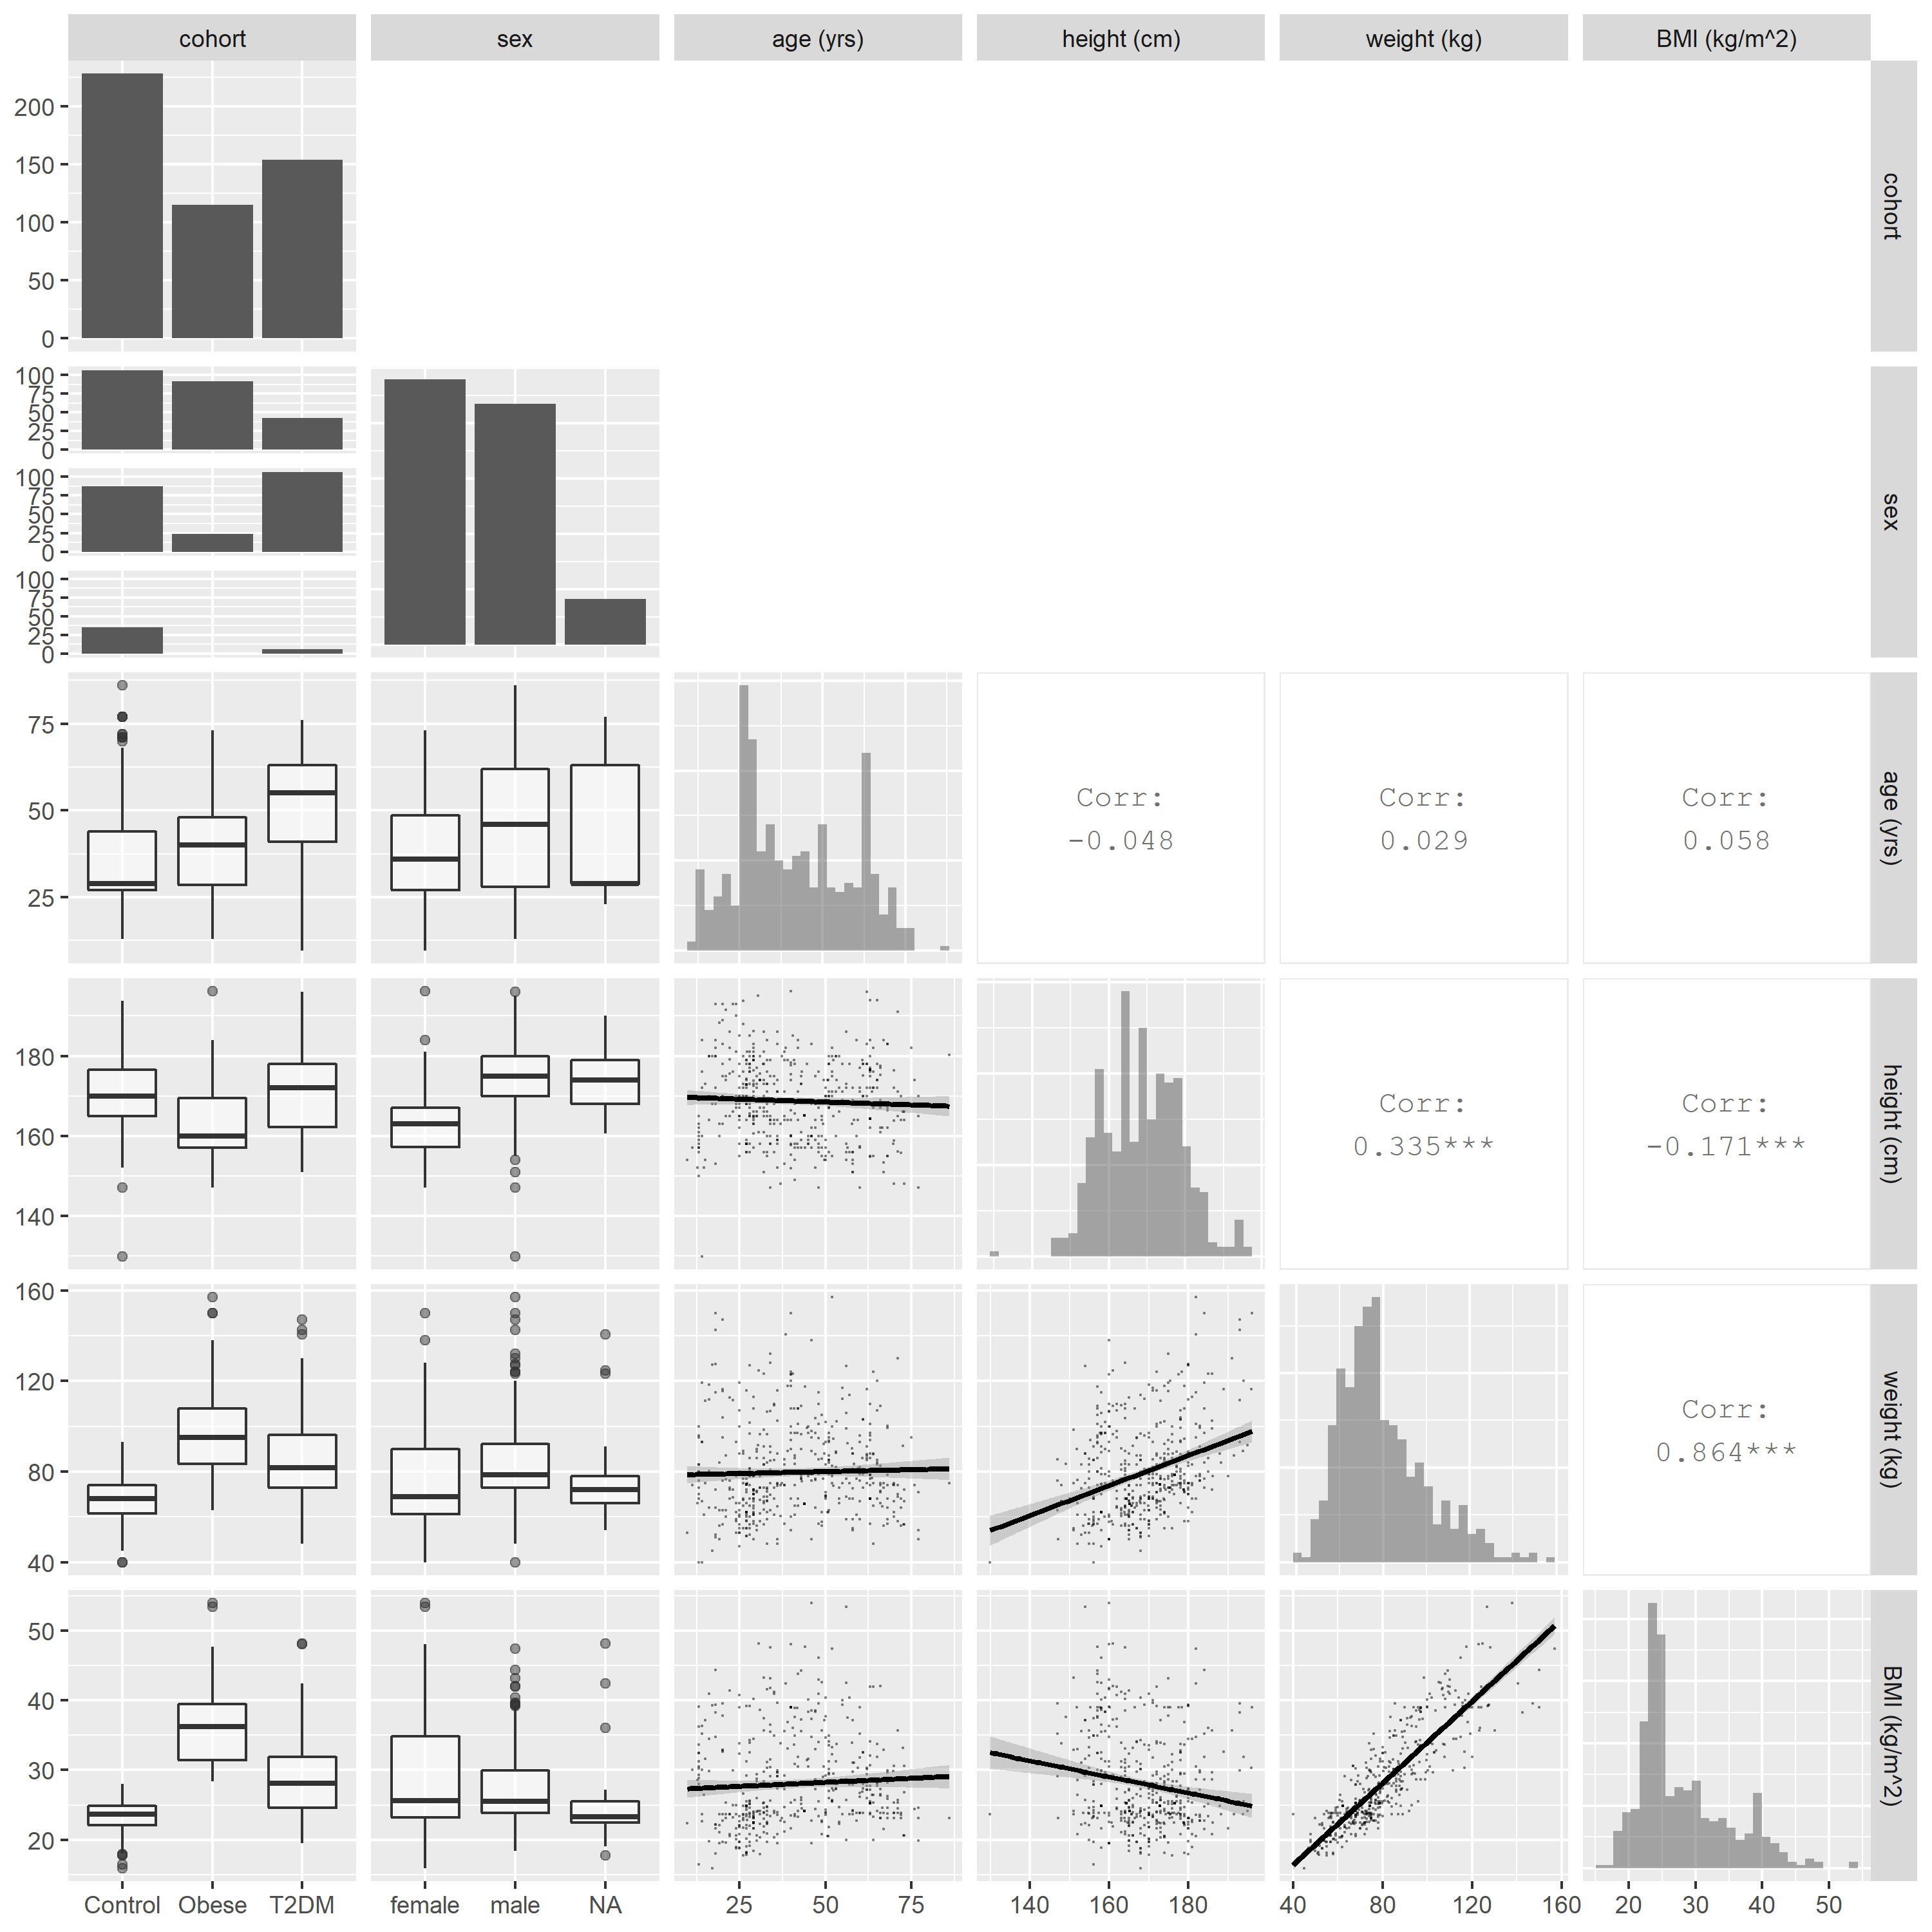
\includegraphics[width=15cm]{p2.PNG}
\end{center}
\caption{Overview of covariate values and relationships. Histograms plots for continuous covariates and bar graphs for discrete covariates are shown on the diagnoal. In the lower triangle, the boxplots between continuous and discrete covariates and scatter plots between continuous covariates are displayed. In the upper triangle, the correlation coefficients between continuous covariates are shown}
\label{fig: cova}
\end{figure}

\begin{figure}[h!]
\begin{center}
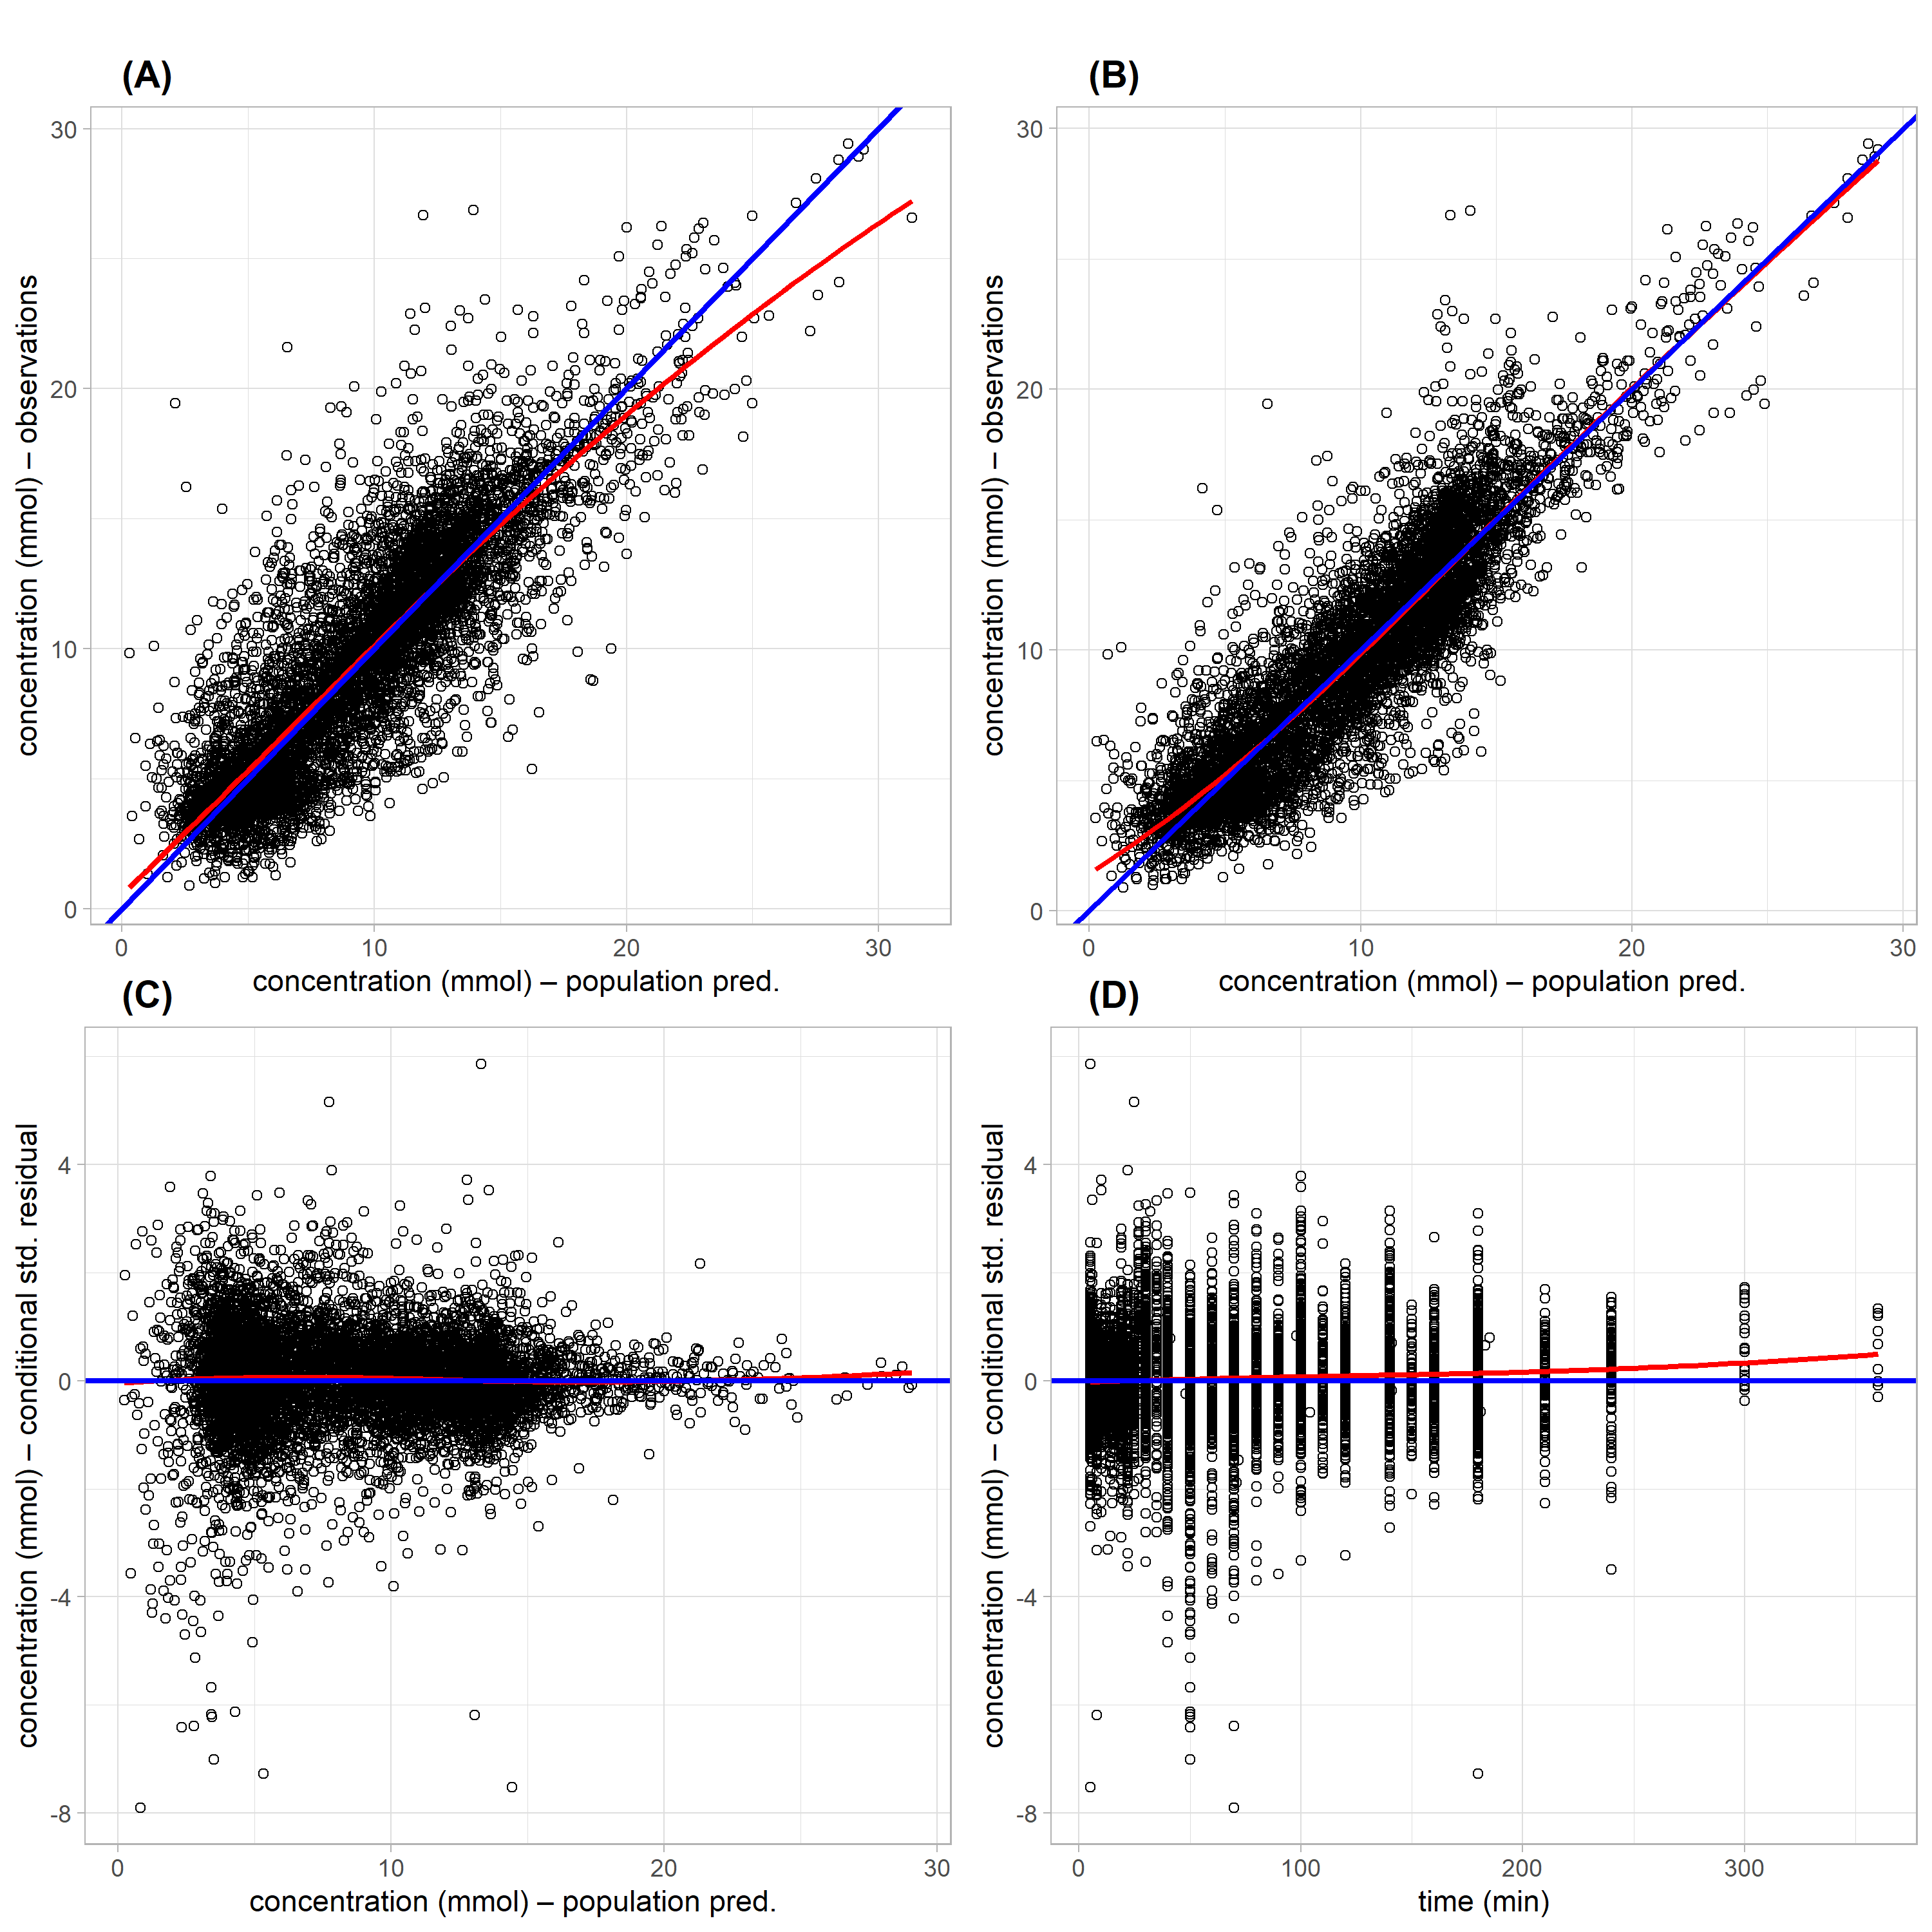
\includegraphics[width=15cm]{comb.PNG}
\end{center}
\caption{Goodness-of-fit plots of the base model without covariates and the final model with covaraites. \textbf{(A)}: observed glucose concentration versus population prediction from the base model. \textbf{(B)}: observed glucose concentration versus population prediction from the final model. \textbf{(C)}: conditional standardized residuals versus population prediction in  the final model. \textbf{(D)}: conditional standardized residual in the final model versus time. Blue lines are the lines of identity or zero value; red lines are loess smooth curves}
\label{fig: fittings}
\end{figure}

\begin{figure}[h!]
\begin{center}
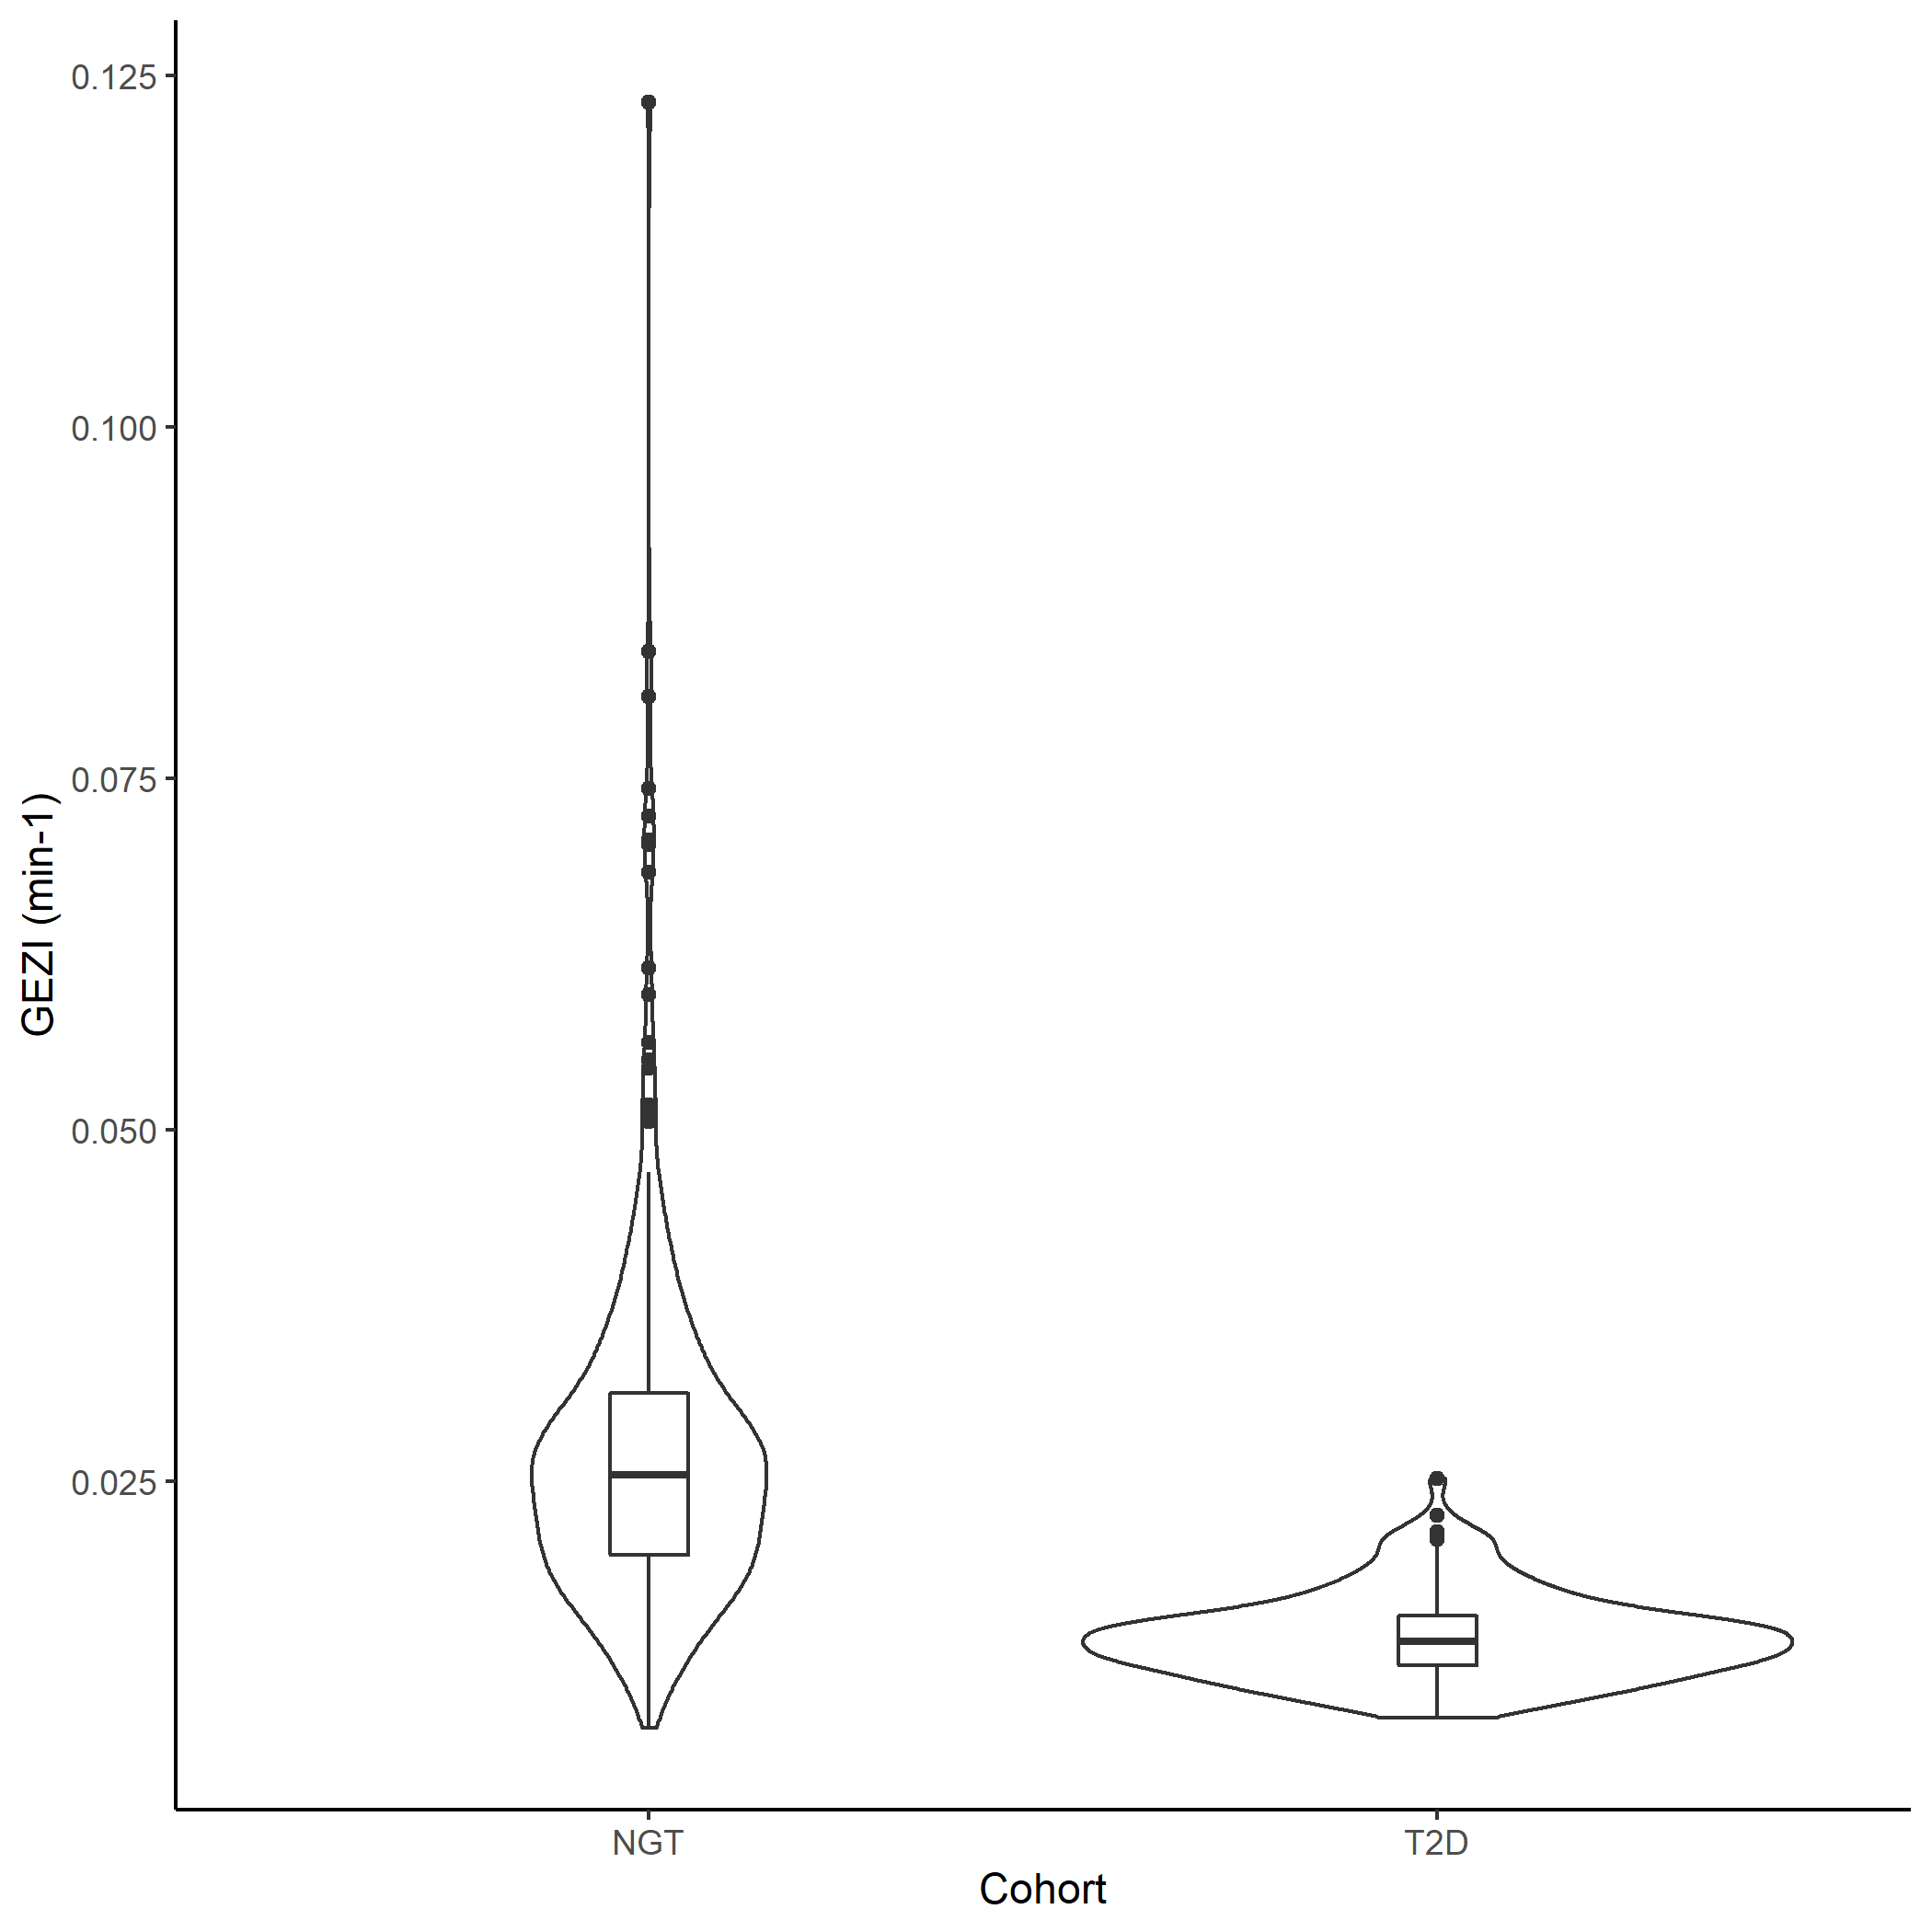
\includegraphics[width=15cm]{SG_co.PNG}
\end{center}
\caption{Violin plots showing the distribution of the individual subjects conditional mean estimates of $GEZI$ in the NGT and T2D cohorts. Boxplots were inserted for each cohort to indicate medians and interquartile ranges}
\label{fig: SG_co}
\end{figure}

\begin{figure}[h!]
\begin{center}
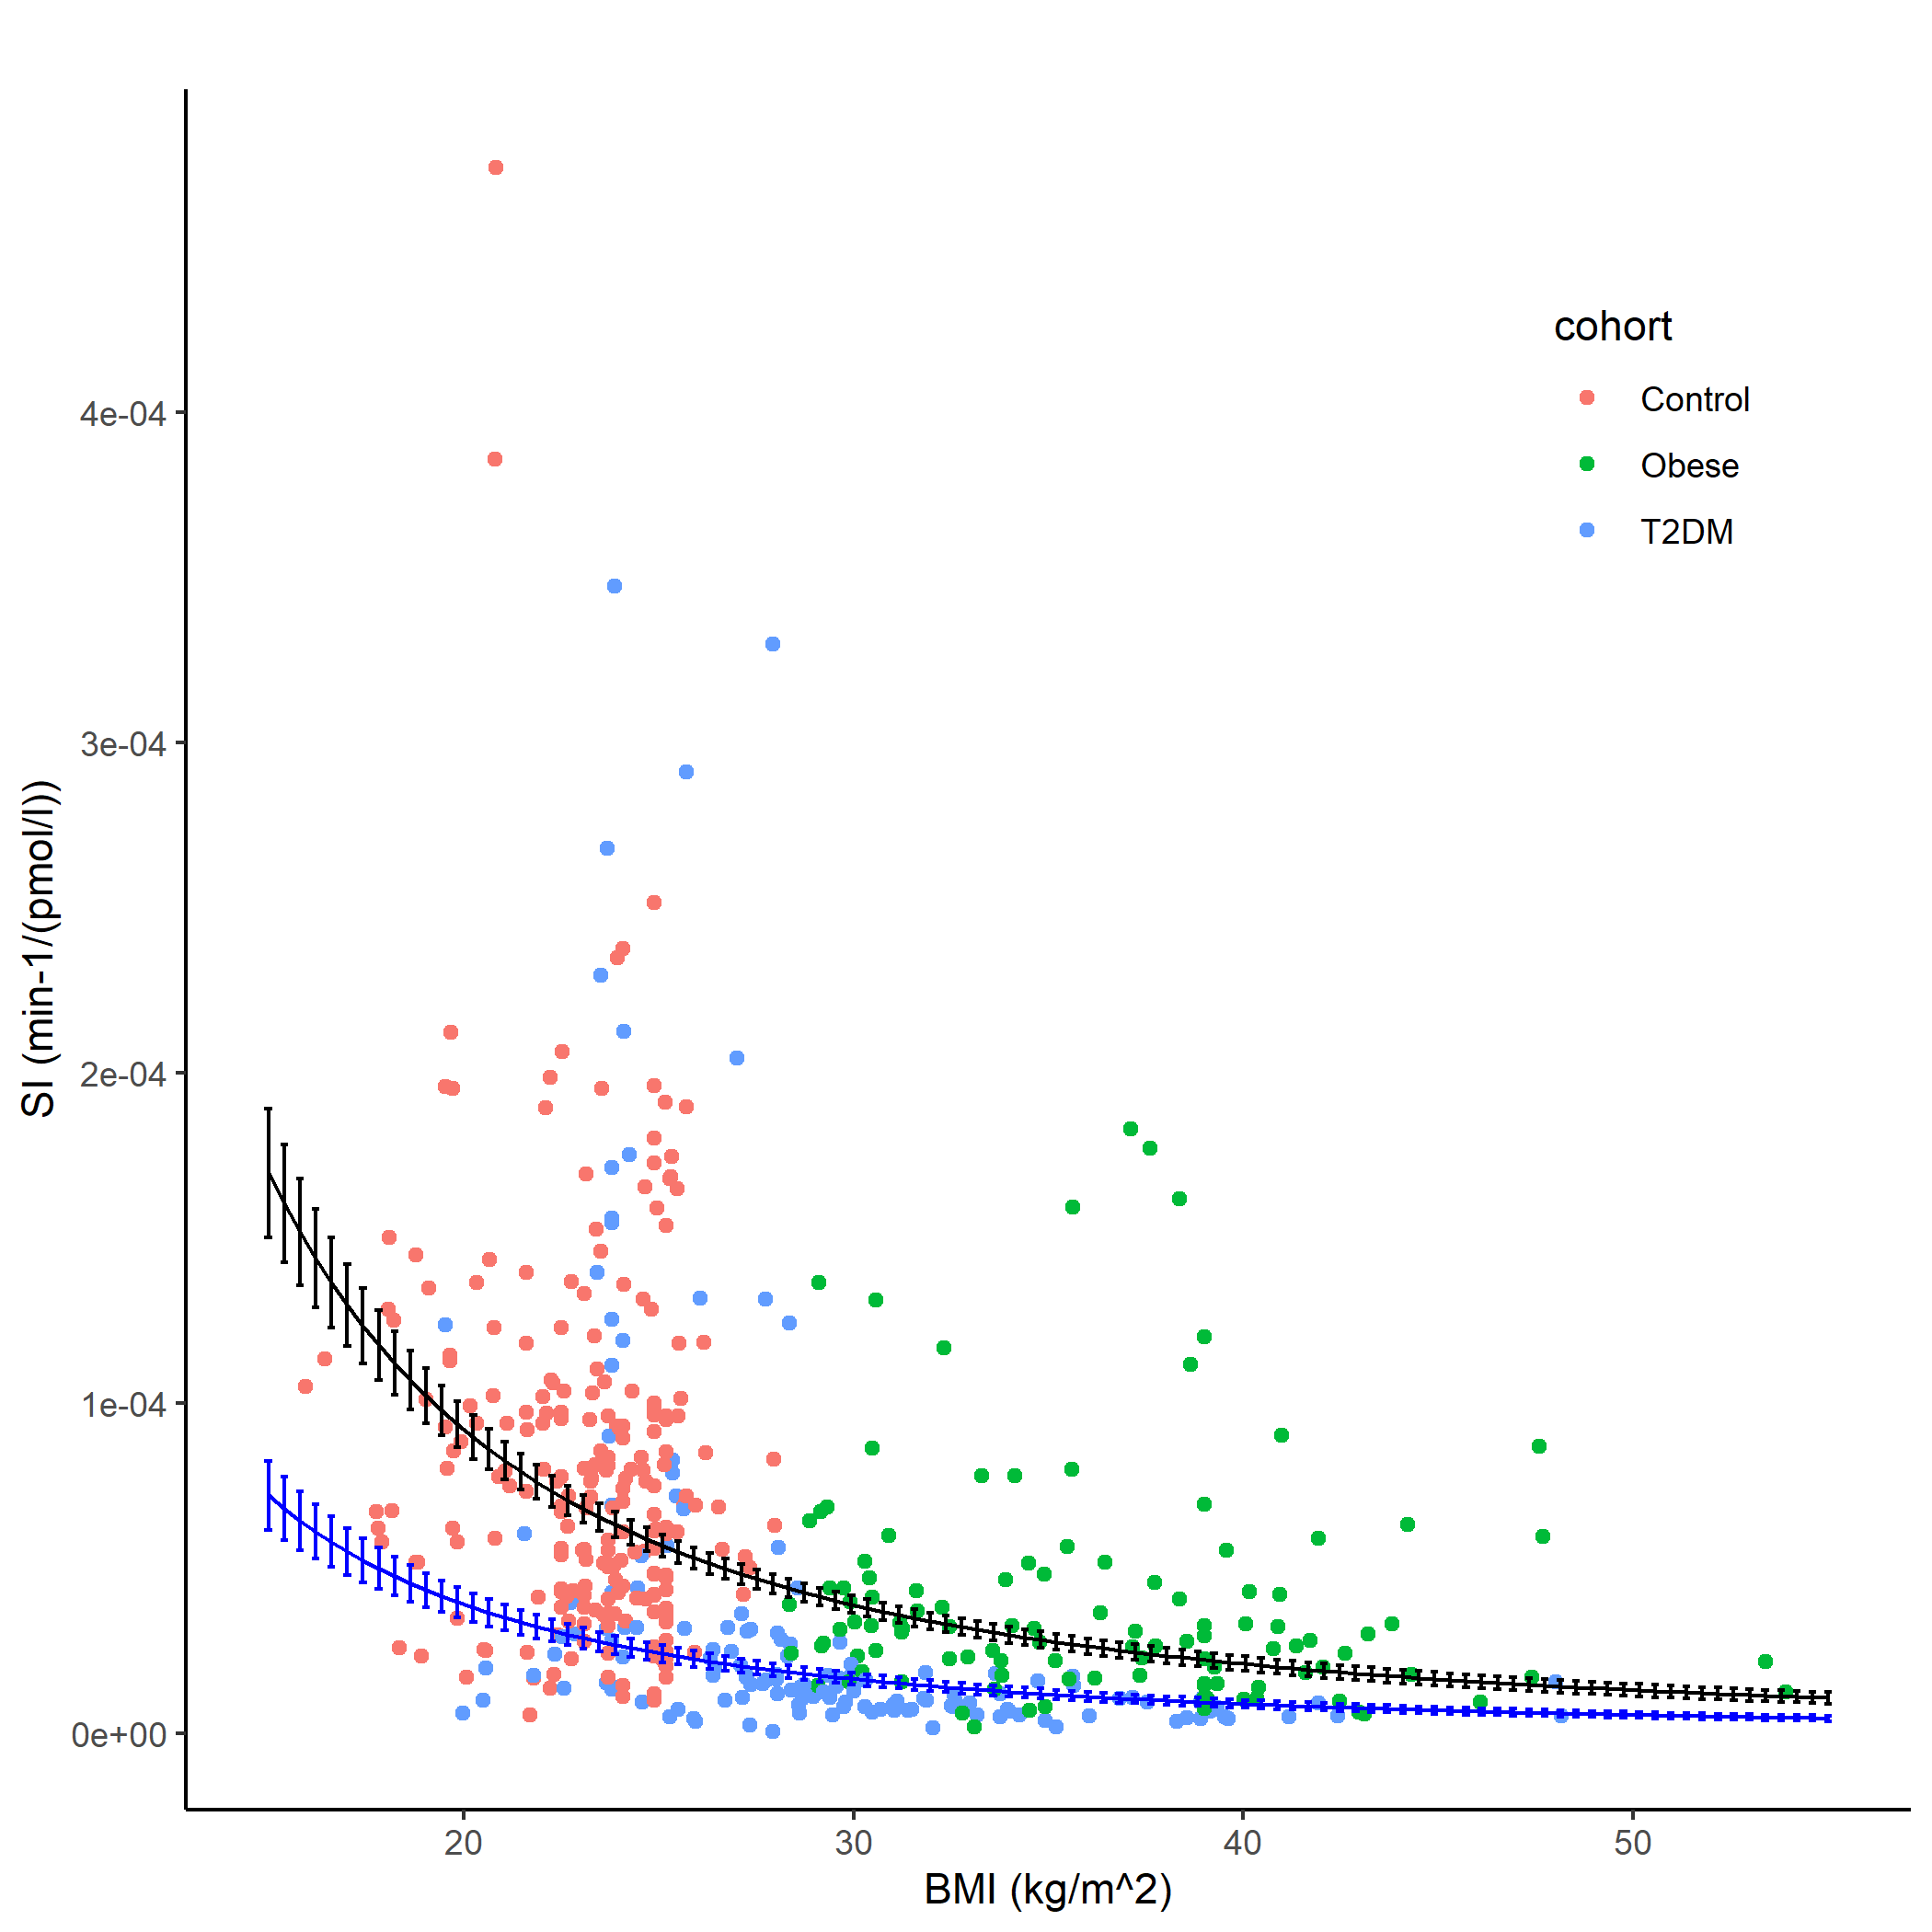
\includegraphics[width=15cm]{SI_BMI.PNG}
\end{center}
\caption{The black line shows the covariatehttps://www.overleaf.com/project/5f7c9af1716f7400018a1fe7 model prediction of the typical value of $S_I$ versus BMI in NGT subjects, while the red line is the corresponding curve in T2D patients. The symbols show the individual subject condition mean estimates of $S_I$ versus their BMI values in NGT (black) and red (T2D) subjects}
\label{fig: SI_BMI}
\end{figure}

%\begin{figure}[h!]
%\begin{center}
%%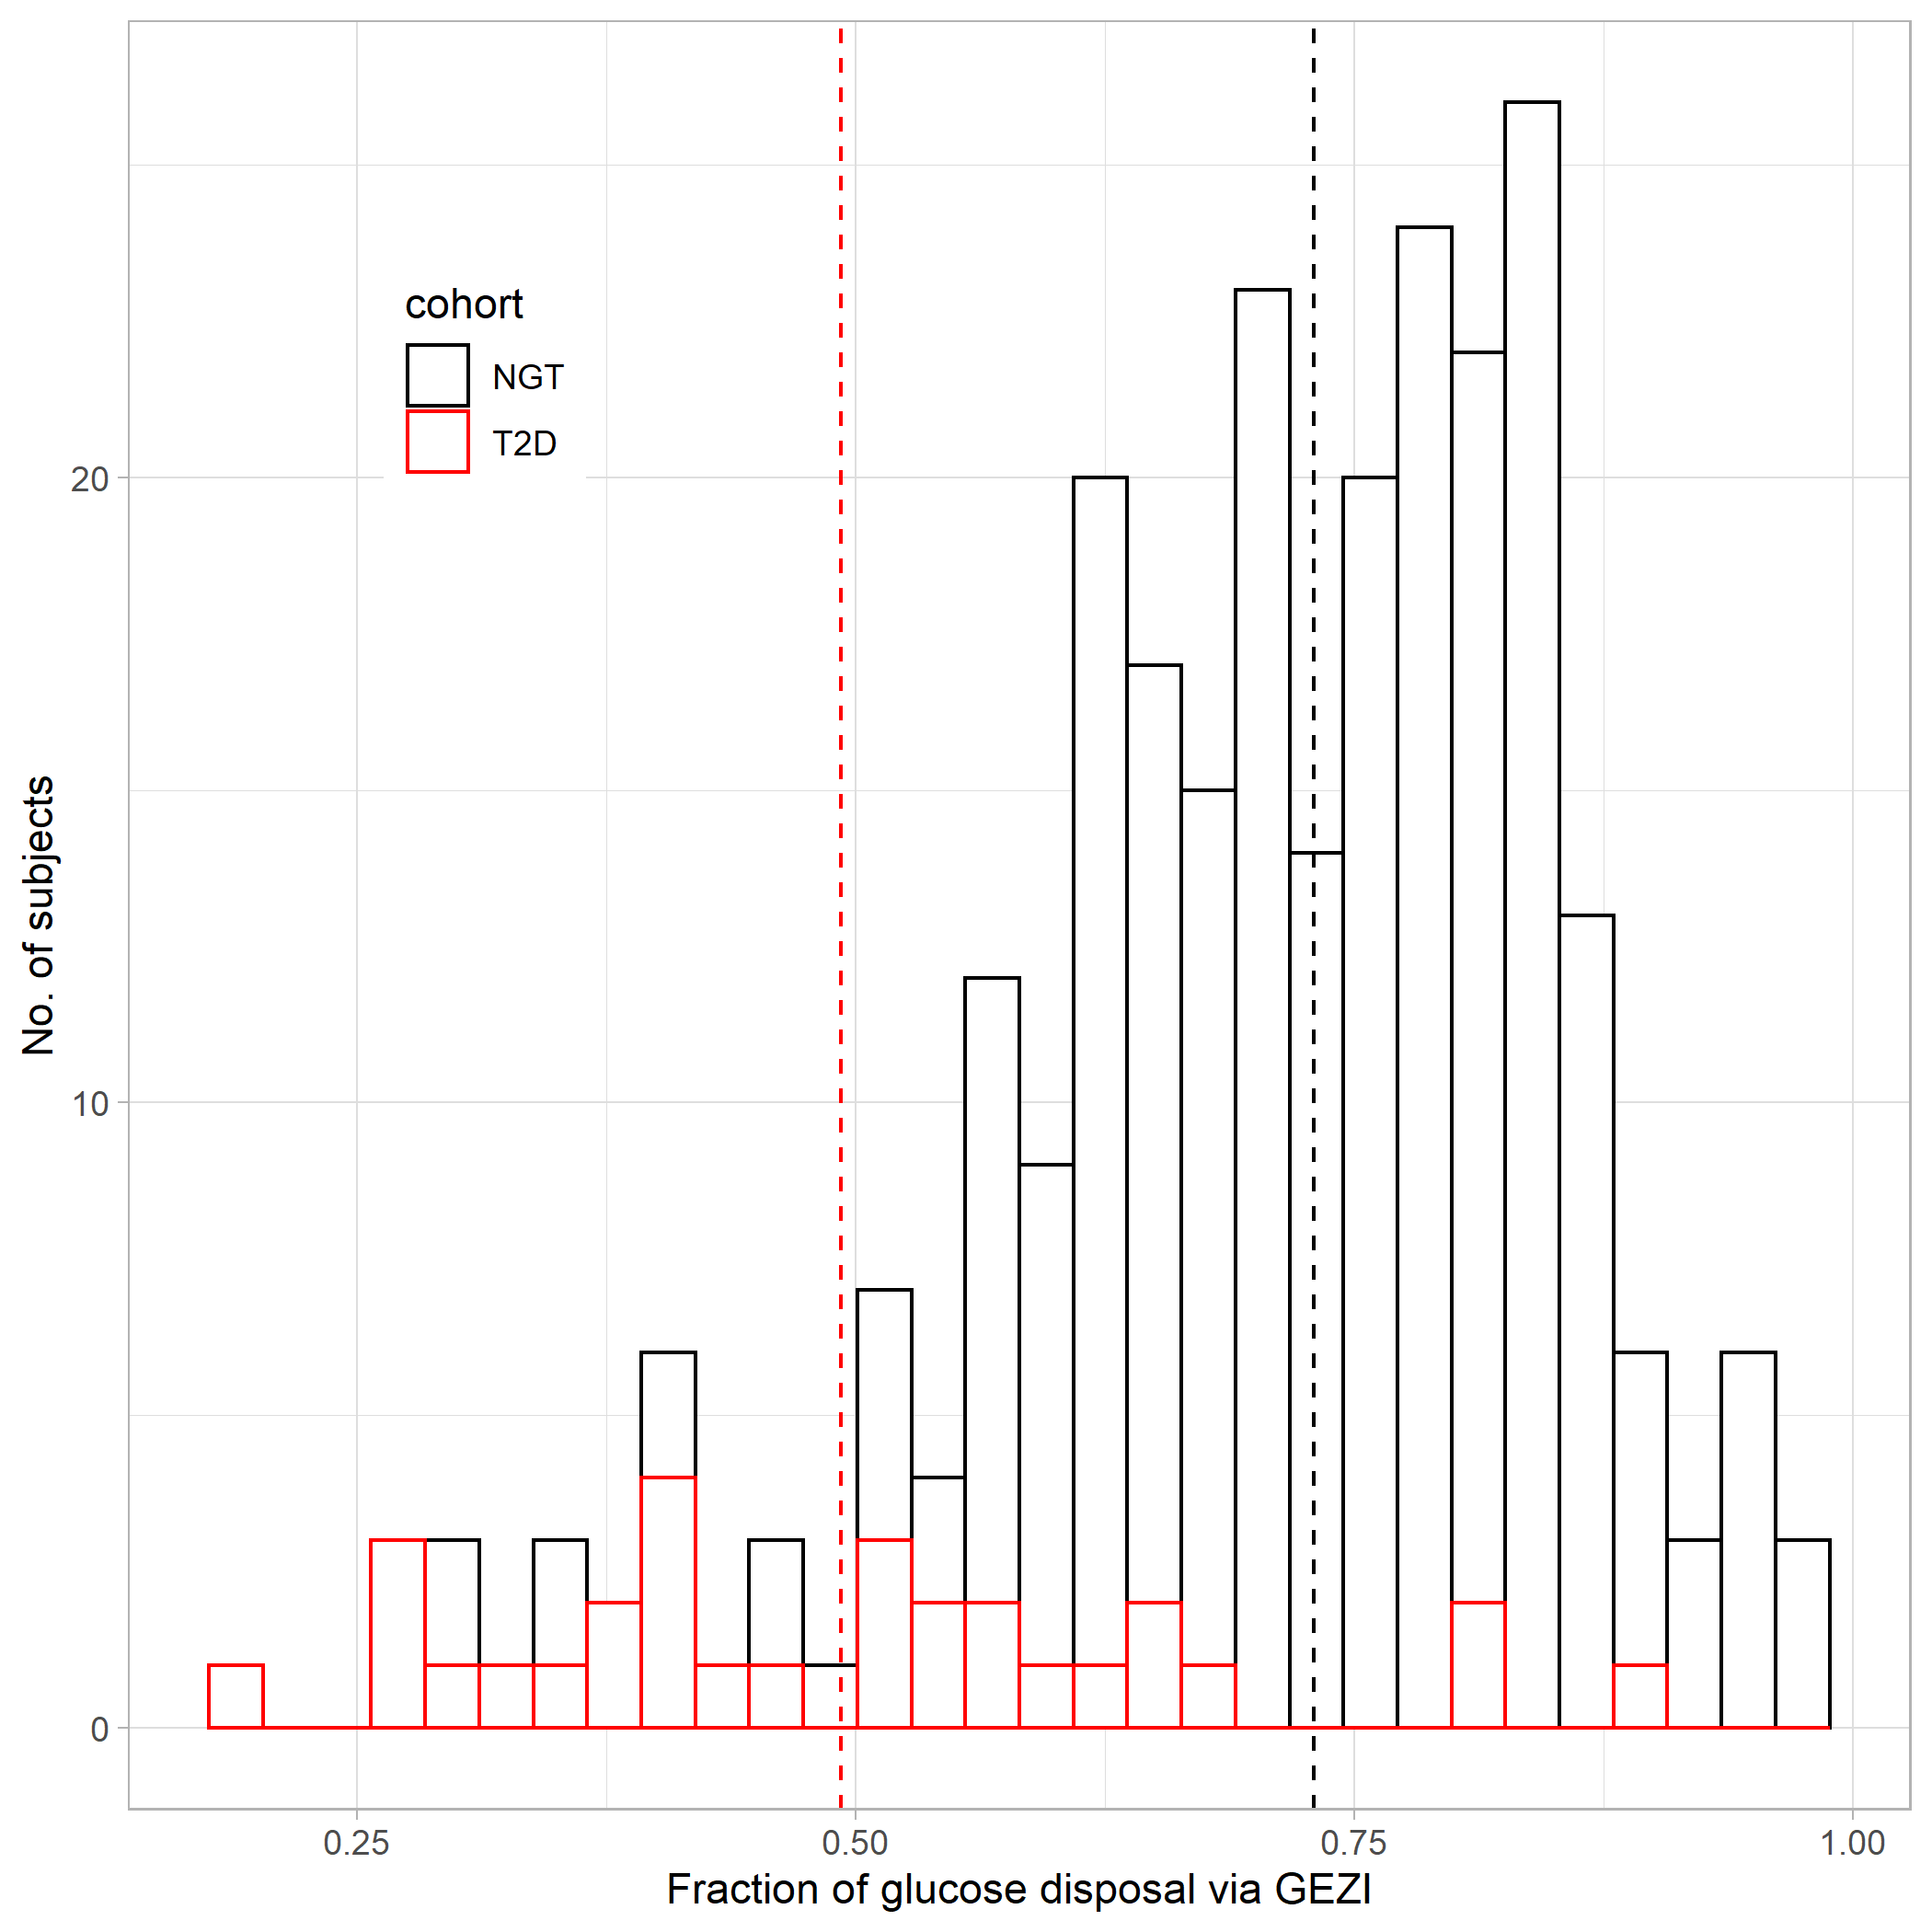
\includegraphics[width=15cm]{frac.PNG}
%\end{center}
%\caption{The histogram showing the distribution of fraction of glucose disposal via GEZI of 497 subjects at the steady state. The bars with black and red outlines indicate 343 NGT and 154 T2D subjects, respectively. The means of the two cohorts are labelled as dash lines}
%\label{fig: frac}
%\end{figure}

\begin{figure}[h!]
\begin{center}
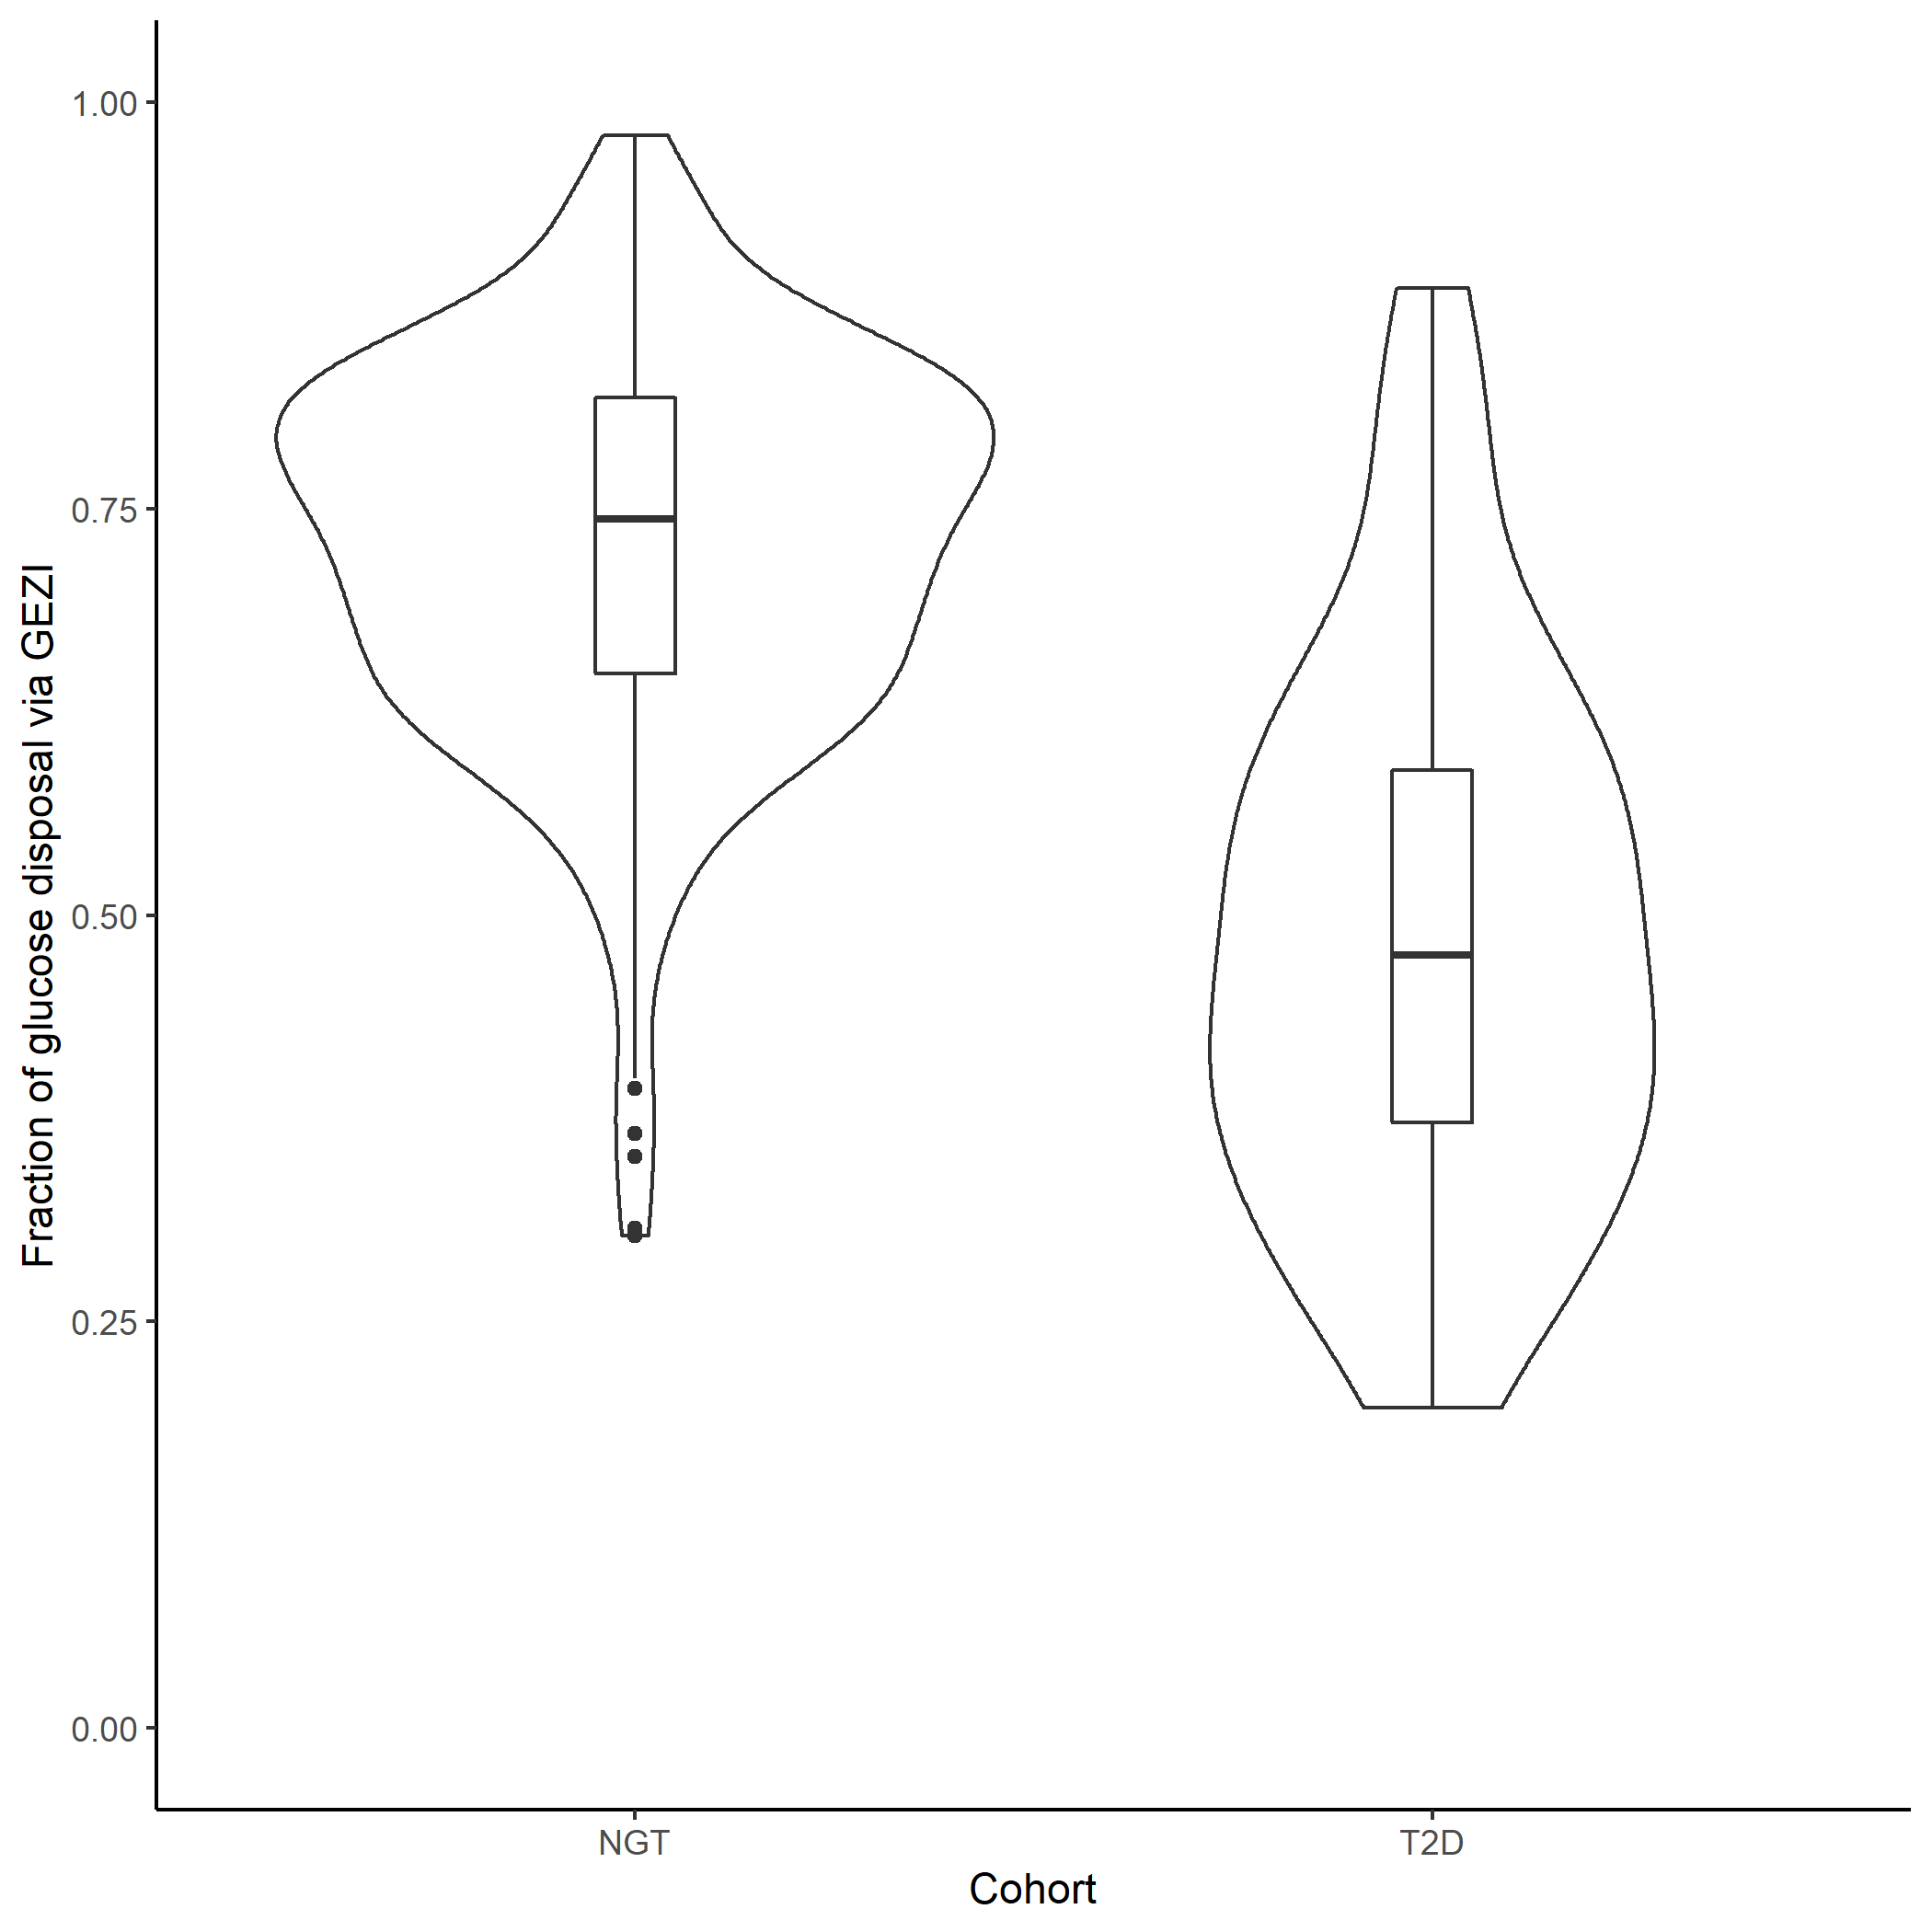
\includegraphics[width=15cm]{frac_IVGTT.PNG}
\end{center}
\caption{Violin plots showing the distribution of the fraction of net glucose disposal via $GEZI$ in 238 NGT subjects and 30 T2D patients. Boxplots were inserted for each cohort to indicate medians and interquartile ranges}
\label{fig: frac}
\end{figure}

%%\begin{figure}[h!]
%%\begin{center}
%%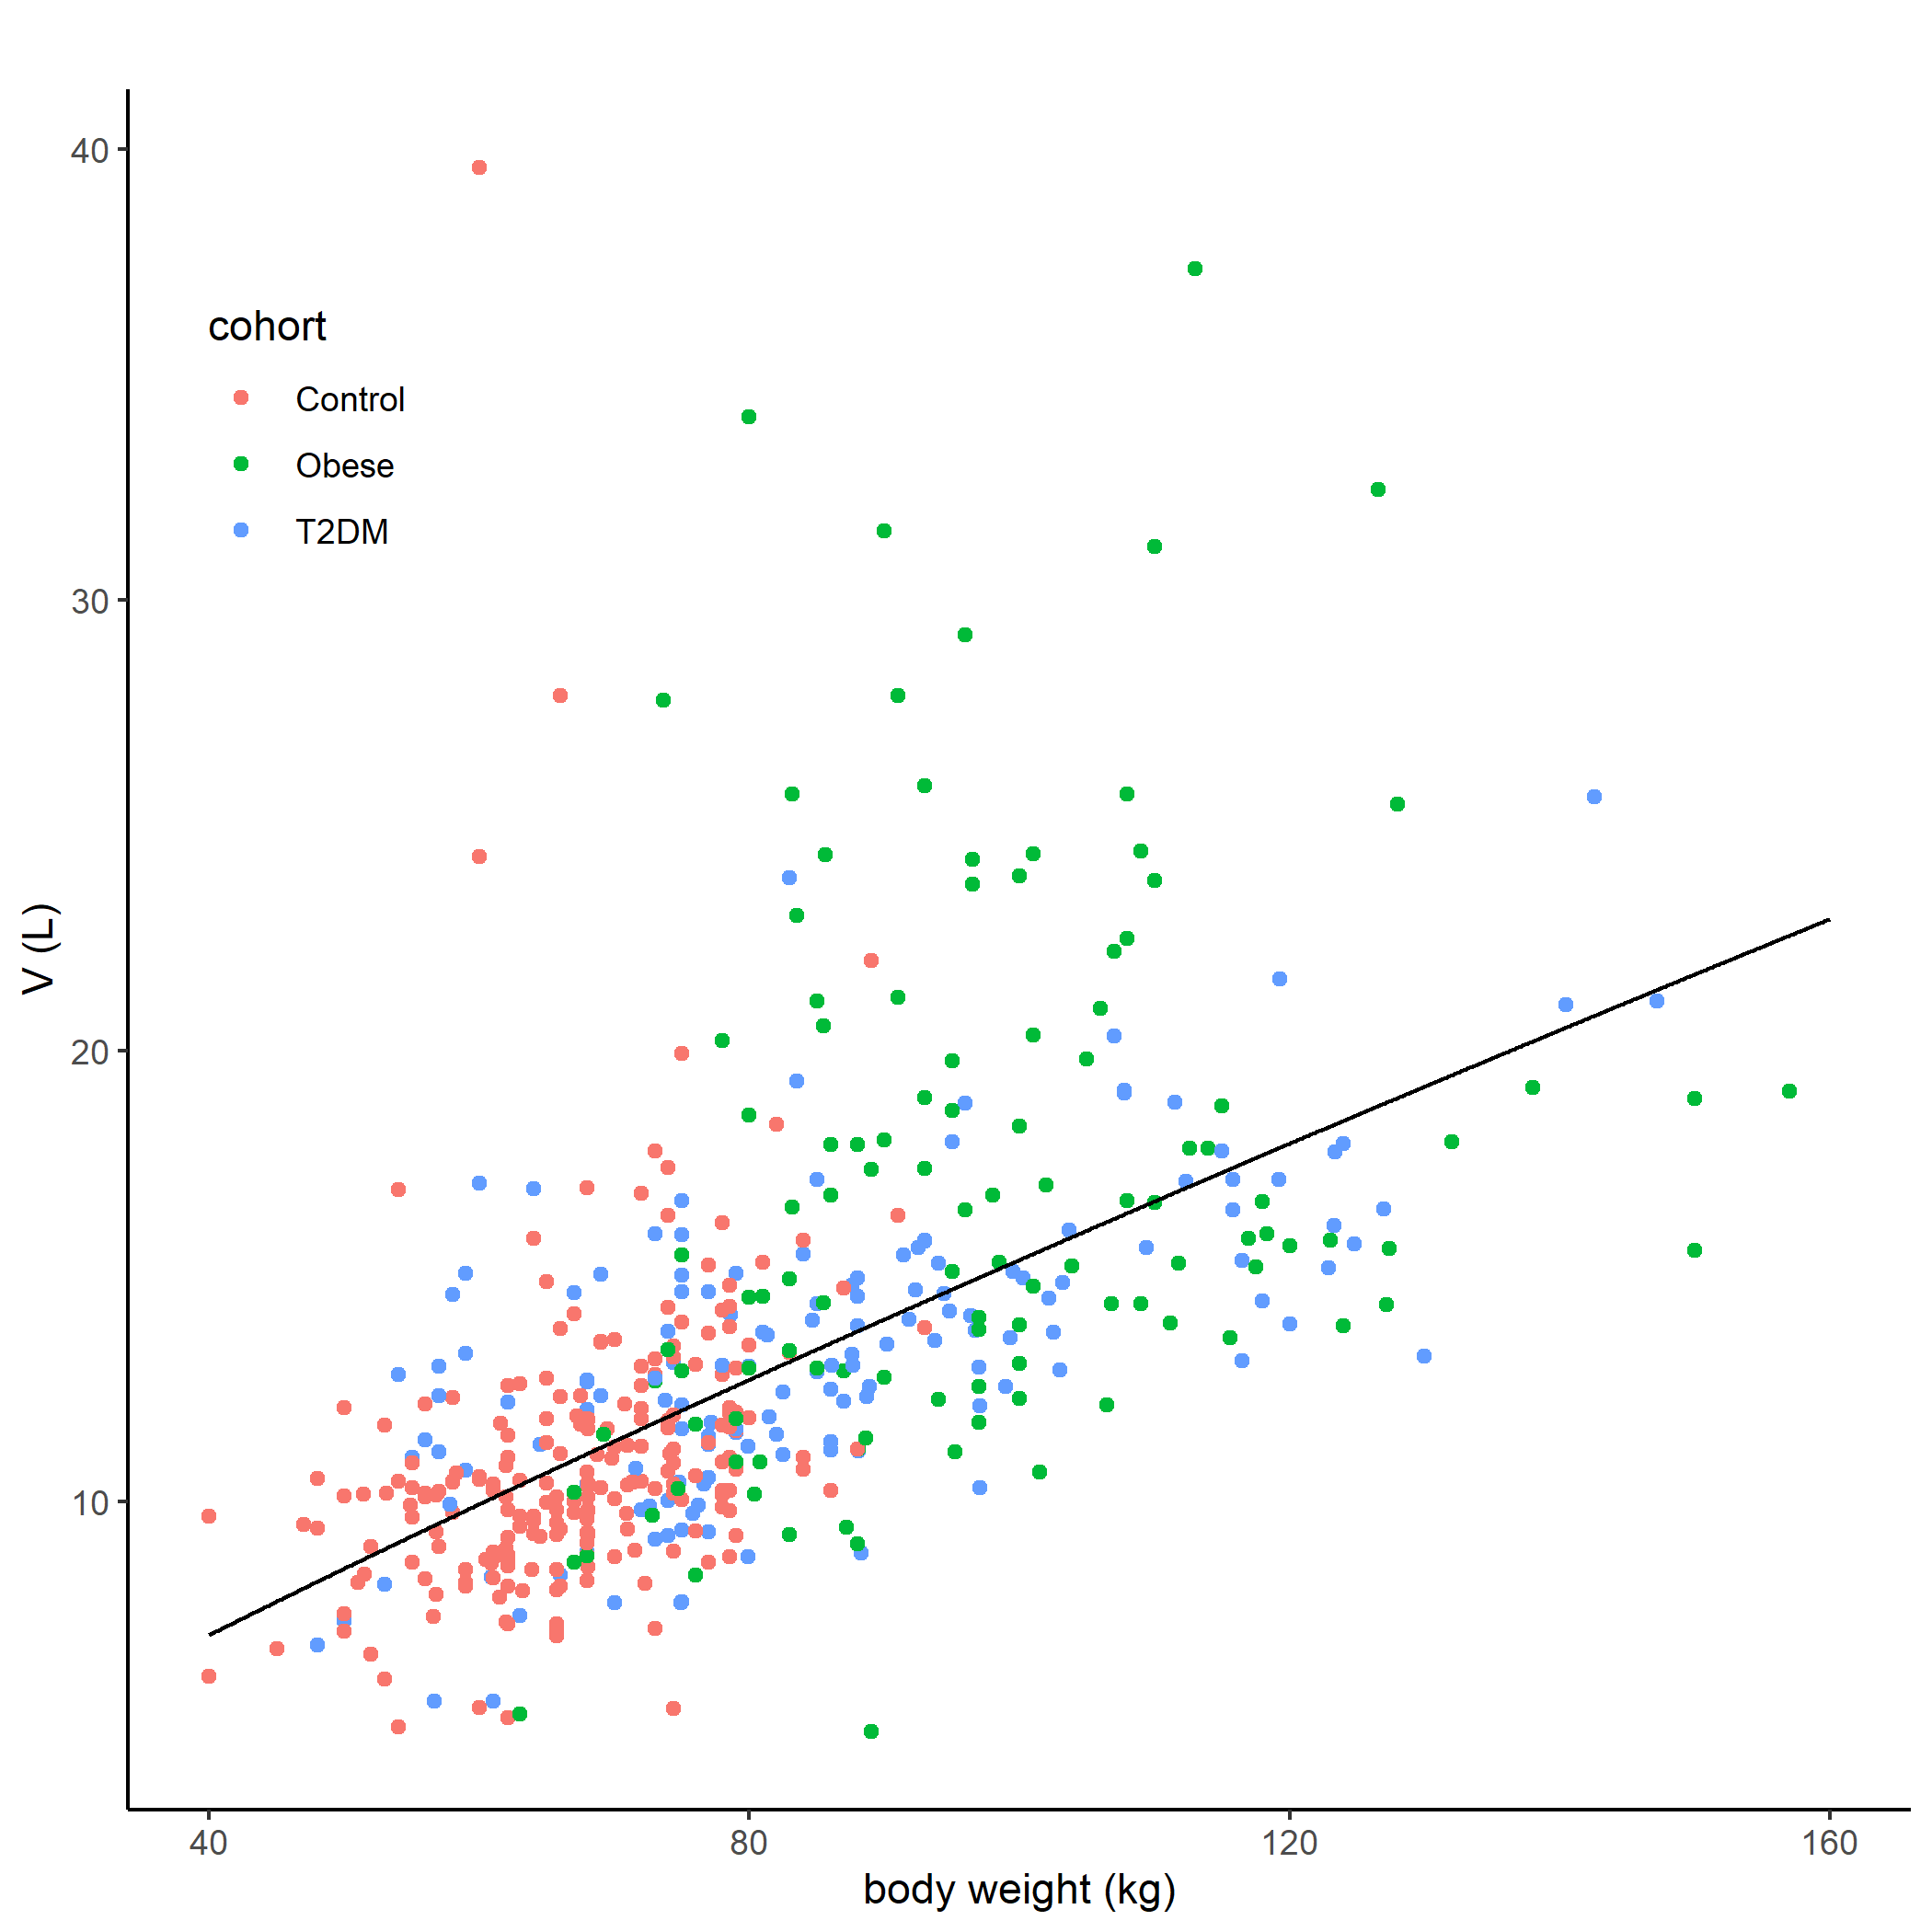
\includegraphics[width=15cm]{V_BW.PNG}
%%\end{center}
%%\caption{Scatter plots and model predicted relationships between $V$ and body weight in NGT and %%T2D cohorts. Dots with different colors display the positive association between $V$ and body %%weight. The black curve shows the model predicted $V$ given the body weight in all the subjects}
%%\label{fig: V_BW}
%%\end{figure}

\end{document}


